% Autor: Alfredo Sánchez Alberca (email:asalber@ceu.es)

% -----------------------------------------------------------------------------------------
%   PREÁMBULO
% -----------------------------------------------------------------------------------------

% Documentclass definition
% Autor: Alfredo Sánchez Alberca (email:asalber@ceu.es)

\documentclass%
[%
paper=a4,  
fontsize=11pt,
DIV=12, 
BCOR=12mm,
headings=big,
parskip=half,
numbers=noendperiod, % 2.3.1 vs 2.3.1. (no dot after the last chapter number)
twoside=true,
bibliography=totoc, % Bibliography appears in Table of Contents (without a number)
toc=listof, % List of Figures and List of Tables appear in Table of Contents
version=last % Use latest version of the KOMA-Script
]%
{scrbook}

% Additional packages of the KOMA-Script family
% Autor: Alfredo Sánchez Alberca (email:asalber@ceu.es)

% Special KOMA-Script package - I added it because I also use the float package in this template, see: 
% http://tex.stackexchange.com/questions/51867/koma-warning-about-toc
% CTAN: http://www.ctan.org/tex-archive/macros/latex/contrib/koma-script/doc
\usepackage{scrhack}

% Better support for marginnotes
% new command: \marginnote
% LaTeX standard command: \marginpar
% CTAN: http://www.ctan.org/pkg/marginnote
\usepackage{marginnote}

% Extended header and footer support
% CTAN: http://www.ctan.org/pkg/scrpage2
\usepackage[%
%  	automark,
%  	ilines,
	headsepline=false
%	footsepline
]{scrpage2}

\pagestyle{scrheadings}
\clearscrheadfoot 
%\ihead{\headmark}
%\ohead[\pagemark]{\pagemark}
\renewcommand*{\pagemark}{%
\usekomafont{pagenumber}%
\ifodd\value{page}%
\makebox[\marginparwidth][l]
{\pnumbar\enskip\thepage}%
\else
\makebox[\marginparwidth][r]
{\thepage\enskip\pnumbar}%
\fi
}

% Page settings (margins, line spacing, indent etc.)
% Autor: Alfredo Sánchez Alberca (email:asalber@ceu.es)

% Márgenes
% \usepackage{geometry}
% \geometry{% 
% 	bottom=30mm,
% 	showframe=false, % For debugging: try true and see the layout frames
% 	margin=30mm,
% 	marginparsep=3mm,
% 	marginparwidth=20mm
% }

% Interlineado
\usepackage{setspace}
\onehalfspacing

% Indentación de la primera línea
\setlength{\parindent}{0.5cm}

% Colors settings
% Autor: Alfredo Sánchez Alberca (email:asalber@ceu.es)

% Soporte para el uso de colores. 
% La opción 'Table': carga también el paquete colortbl para colorear filas, columnas y celdas de tablas.
\usepackage[table]{xcolor} 
\definecolor{color1}{RGB}{80,187,48}
\definecolor{color2}{RGB}{174,49,54}
\definecolor{ocre}{RGB}{243,102,25} % Define the orange color used for highlighting throughout the book
\definecolor{blueceu}{RGB}{5,161,230} % Blue color of CEU logo
\definecolor{greenceu}{RGB}{185,209,16} % Green color of CEU logo
\definecolor{redceu}{RGB}{137,28,36} % Red color of CEU logo
\definecolor{purpleceu}{RGB}{169,78,145} % Purple color of CEU log
\definecolor{grayceu}{RGB}{111,107,83} % Gray color of CEU logo
\definecolor{coral}{rgb}{1,0.5,0.31} % Orange color for graphics
\definecolor{royalblue1}{rgb}{0.28,0.46,1} % Blue color for graphics
\definecolor{mygreen}{rgb}{0,0.8,0} % Green color for graphics
\definecolor{chaptergrey}{RGB}{5,161,230} % Blue color of CEU logo
\definecolor{mygray}{gray}{0.2}


% Common packages
% Author: Alfredo Sánchez Alberca (email:asalber@ceu.es)
% 
% UTF8 encoding
\usepackage[utf8]{inputenc}

% T1 font encoding
\usepackage[T1]{fontenc}

% Font 
%\usepackage[libertine,cmintegrals,cmbraces,vvarbb]{newtxmath}
\usepackage[sc]{mathpazo}
% Improve the font visualization in pdf
\usepackage{microtype} 

% Language support
\usepackage[english]{babel} 

% AMS support 
\usepackage{amsmath}
\usepackage{amssymb}
\usepackage{mathtools}

% Euro symbol
\usepackage{eurosym}

% Math calculations support
\usepackage{calc}

% Extended support for graphics
\usepackage{graphicx}

% Adjust width and heigh of boxes (and images)
\usepackage[export]{adjustbox}

% Better suport for alingning to the left and right with the commands \RaggedRight and \RaggedLeft. 
\usepackage{ragged2e}

% Vectorial plots
\usepackage{tikz}
\usetikzlibrary{shapes,arrows,positioning,decorations.pathreplacing,trees}

% Facilities fo define macros
\usepackage{etoolbox}

% Inclusion of pdf
\usepackage{pdfpages}
 

% List settings
% Autor: Alfredo Sánchez Alberca (email:asalber@ceu.es)

% Listas
\usepackage[inline]{enumitem}
\setlist[1]{labelindent=\parindent} % Indentación de listas de primer nivel igual que la primera linea de párrafo

% Listas de descripción justificadas con la etiqueta que se especifique en el parámetro 
\newenvironment{descriptionvar}[1]{
\begin{list}{}{
  \renewcommand{\makelabel}[1]{\textbf{##1}\hfil}
  \settowidth{\labelwidth}{\textbf{#1}}
  \setlength{\leftmargin}{\labelwidth}\addtolength{\leftmargin}{\labelsep}}
}
{\end{list}}

% Tables settings
% Autor: Alfredo Sánchez Alberca (email:asalber@ceu.es)

% Tablas bonitas
\usepackage{booktabs}

% Tablas balanceadas
\usepackage{array}
\usepackage{tabularx}
\usepackage{tabulary}
\newcolumntype{Y}{>{\raggedleft\arraybackslash}X}

% Tablas grandes
\usepackage{longtable}

% Color en tablas
%\usepackage{colortbl} Caragada por le paquete xcolor con la opción table
\newcommand{\tcrule}{\arrayrulecolor{color1!50!white}\toprule}
\newcommand{\mcrule}{\arrayrulecolor{color1!50!white}\midrule}
\newcommand{\bcrule}{\arrayrulecolor{color1!50!white}\bottomrule}

% Fusión de filas en tablas
\usepackage{multirow}

% Rotación de tablas
\usepackage{pdflscape}

% Theorems settings
% Autor: Alfredo Sánchez Alberca (email:asalber@ceu.es)

% Teoremas en cajas coloreadas
\usepackage[most]{tcolorbox}
\tcbuselibrary{minted}
\usepackage{varwidth}
 
\DeclareTotalTCBox{\tcverb}{m}{nobeforeafter, tcbox raise base, size=fbox}{\texttt{#1}}
%\newtcbox{\tcverb}{nobeforeafter,verbatim,tcbox ,size=fbox,height=\baselineskip}

%\DeclareTotalTCBox{\tcverb}{s v}{verbatim}{\lstinline[language=command.com]^#2^}


\newtcbox{cajapeque}{nobeforeafter, tcbox raise base}
\newtcolorbox{cajagrande}{}

% Listado de código no numerado. El primer parámetro es opcional e indica el lenguaje y el segundo es obligatorio e indica el
% título
\DeclareTCBListing{listado}{O{} m}{%
breakable,
noparskip,
listing engine=minted,
listing only,
list entry={\protect\numberline{\thetcbcounter}#3},
colback=red!5!white,
colframe=red!75!black,
fonttitle=\bfseries,
title=#2,
minted language=#1}

% Listado de código númerado. Ël primer parámetro es opcional e indica el lenguaje y el segundo es obligatorio e indica el título
% \DeclareTCBListing{listadonum}{O{} m}{%
% enhanced,
% breakable,
% noparskip,
% listing engine=minted,
% minted options={fontsize=\small,linenos,numbersep=2mm},
% listing only,
% colback=red!5!white,
% colframe=red!75!black,
% fonttitle=\bfseries,
% title=#2,
% minted language=#1,
% overlay={\begin{tcbclipinterior}\fill[red!20!blue!20!white] (frame.south west)
% rectangle ([xshift=5mm]frame.north west);\end{tcbclipinterior}}}

\newtcblisting[auto counter,number within=chapter, list inside=listado]{listadonum}[3][turtle]{
enhanced,
breakable,
noparskip,
listing engine=minted,
minted options={fontsize=\small,linenos,numbersep=2mm},
listing only,
list entry={\protect\numberline{\thetcbcounter}#2},
colback=red!5!white,
colframe=red!75!black,
fonttitle=\bfseries,
title={Listado \thetcbcounter: #2},
label={list:#3},
minted language=#1,
overlay={\begin{tcbclipinterior}\fill[red!20!blue!20!white] (frame.south west)
rectangle ([xshift=5mm]frame.north west);\end{tcbclipinterior}}}


\newtcbtheorem[auto counter, number within=chapter, list inside=tabla]{tabla}{Tabla}{
enhanced,
breakable,
left=0mm,
right=0mm,
top=0mm,
bottom=0mm,
boxsep=1mm,
toptitle=1mm,
bottomtitle=1mm,
fonttitle=\bfseries,
colback=yellow!10!white,
colframe=color1!50!white,
coltitle=color1!50!black,
list entry={\protect\numberline{\thetcbcounter}#2},
}{tab}


\newtcbtheorem[number within=chapter]{teorema}{Teorema}{
enhanced,
breakable,
frame empty,
colback=greenceu!10!white,
colframe=color1!50!white,
coltitle=color1!50!black,
colbacktitle=color1!15!white,
fonttitle=\bfseries,
top= 5mm,
borderline={0.5mm}{0mm}{color1!50!white},
attach boxed title to top left={yshift=-3mm, xshift=5mm },
boxed title style={boxrule=0.4pt},
varwidth boxed title
}{teo}


\newtcbtheorem[number within=chapter]{definicion}{Definición}{
enhanced,
breakable,
frame empty,
colback=greenceu!10!white,
colframe=color1!50!white,
coltitle=color1!50!black,
colbacktitle=color1!15!white,
fonttitle=\bfseries,
top= 5mm,
borderline={0.5mm}{0mm}{color1!50!white},
attach boxed title to top left={yshift=-3mm, xshift=5mm },
boxed title style={boxrule=0.4pt},
varwidth boxed title
}{def}


\newtcbtheorem[number within=chapter]{ejemplo}{Ejemplo}{
enhanced,
breakable,
frame empty,
%colback=greenceu!10!white,
colframe=color2!50!white,
coltitle=color2!50!black,
colbacktitle=color2!15!white,
fonttitle=\bfseries,
top= 5mm,
borderline={0.5mm}{0mm}{color2!50!white},
attach boxed title to top left={yshift=-3mm, xshift=5mm },
boxed title style={boxrule=0.4pt},
varwidth boxed title
}{ej}


% \newtcbtheorem[number within=chapter]{ejemplo}{Ejemplo}{
% enhanced,
% breakable,
% skin=enhancedlast jigsaw,
% attach boxed title to top left={xshift=-4mm,yshift=-0.5mm},
% fonttitle=\bfseries\sffamily,
% varwidth boxed title=0.7\linewidth,
% colbacktitle=color1!15!white,
% coltitle=color1!50!black,
% colframe=color1!50!white,
% %interior style={top color=blue!10!white,bottom color=red!10!white},
% boxed title style={empty,arc=0pt,outer arc=0pt,boxrule=0pt},
% underlay boxed title={
% \fill[color1!50!white] (title.north west) -- (title.north east) -- +(\tcboxedtitleheight-1mm,-\tcboxedtitleheight+1mm) --
% ([xshift=4mm,yshift=0.5mm]frame.north east) -- +(0mm,-1mm) -- (title.south west) -- cycle; 
% \fill[color1!15!white!50!black] ([yshift=-0.5mm]frame.north west) -- +(-0.4,0) -- +(0,-0.3) -- cycle;
% \fill[color1!15!white!50!black] ([yshift=-0.5mm]frame.north east) -- +(0,-0.3) -- +(0.4,0) -- cycle; }
% }{ej}

 

% Table of contents settings
% Autor: Alfredo Sánchez Alberca (email:asalber@ceu.es)

% Level for numbered captions
\setcounter{secnumdepth}{3}

% Level of chapters that appear in Table of Contents
\setcounter{tocdepth}{3} 
% -2 no caption at all
% -1 part
% 0  chapter
% 1  section    
% 2  subsection 
% 3  subsubsection
% 4  paragraph
% 5  subparagraph

% KOMA-Script code to adjust TOC
\makeatletter
\addtokomafont{chapterentrypagenumber}{\large\normalfont\color{color1}}
\addtokomafont{chapterentry}{\large\normalfont\color{color1}}
\makeatother


% Floating evironments settings
% Author: Alfredo Sánchez Alberca (email:asalber@ceu.es)

% Captions support for floating environments
\usepackage[%
	font={small},
	labelfont={bf,sf},
	format=hang, % try plain or hang
	margin=10mm,
]{caption}

% Extended support for floatings 
% \begin{figure}[H]) places the floating environment exactly in the command place.
\usepackage{float}

% Section header settings
% Autor: Alfredo Sánchez Alberca (email:asalber@ceu.es)

% Citas en los capítulos
%\usepackage[palatino]{quotchap}
%\makeatletter
% \renewcommand*{\sectfont}{\Huge\bfseries}
% \renewcommand*{\chapnumfont}{%
%  \usefont{T1}{\@defaultcnfont}{b}{n}\fontsize{120}{150}\selectfont% Default: 100/130
%  \color{chaptergrey}%
% }
%\makeatother

\usepackage{titlesec}

\setkomafont{chapter}{\usefont{T1}{ppl}{b}{n}\fontsize{1cm}{1em}\selectfont\color{color1}} % "ppl" - Font Palatino, "b" -
% negrita
\setkomafont{section}{\usefont{T1}{ppl}{b}{n}\selectfont\LARGE}
\addtokomafont{subsection}{\color{color1}}
\addtokomafont{subsubsection}{\color{color1}}
\addtokomafont{paragraph}{\color{color1}}
\addtokomafont{subparagraph}{\color{color1}}


\titleformat{\chapter}
  {\usekomafont{chapter}} 
  {} % etiqueta
  {0pt} % separación horizontal entre la etiqueta y el cuerpo del título
  {
  \begin{tikzpicture}[remember picture,overlay]
    \node[yshift=-7cm] at (current page.north east) 
      {\begin{tikzpicture}[remember picture, overlay]
        \draw[color1, fill=color1] (-6,0) rectangle (6cm,3cm);
        %\node[anchor=east,xshift=\paperwidth-3cm, yshift=1.5cm] {\color{color2}#1};
		\node[anchor=east,xshift=-3cm, yshift=1.5cm] {\fontsize{3cm}{1em}\selectfont\color{white}\thechapter};
       \end{tikzpicture}
      };
   \end{tikzpicture}
   \hspace{-25pt}
  }
  
\titlespacing*{\chapter}{0pt}{7cm}{2cm}  

\titleformat{name=\chapter,numberless}
  {\usekomafont{chapter}} 
  {} % etiqueta
  {0pt} % separación horizontal entre la etiqueta y el cuerpo del título
  {}

\titlespacing*{name=\chapter,numberless}{0pt}{2cm}{2cm}  

\titleformat{\section}[hang]
  {\usekomafont{section}} % "qhv" - TeX Gyre Heros, "b" - negrita
  {} % etiqueta
  {0em} % separación horizontal entre la etiqueta y el cuerpo del título
  {\color{color1}\thesection\hspace{0.6em}} %código que precede al título
  [] % código opcional que sigue al título
  
\titlespacing*{name=\section}{0pt}{1cm}{0cm}  

\titleformat{\subsection}[hang]
  {\usefont{T1}{ppl}{b}{n}\selectfont} % "qhv" - TeX Gyre Heros, "b" - negrita
  {} % etiqueta
  {0em} % separación horizontal entre la etiqueta y el cuerpo del título
  {\Large \color{color1}\thesubsection\hspace{0.6em}} %código que precede al título
  [] % código opcional que sigue al título
  
\titlespacing*{name=\subsection}{0pt}{0.5cm}{0cm}  

\titleformat{\subsubsection}[hang]
  {\usefont{T1}{ppl}{b}{n}\selectfont} % "qhv" - TeX Gyre Heros, "b" - negrita
  {} % etiqueta
  {0em} % separación horizontal entre la etiqueta y el cuerpo del título
  {\large \color{color1}\thesubsection\hspace{0.6em}} %código que precede al título
  [] % código opcional que sigue al título

\titlespacing*{name=\subsubsection}{0pt}{0.4cm}{0cm} 


% Header and footer settings
% Autor: Alfredo Sánchez Alberca (email:asalber@ceu.es)

% Fuente 
\setkomafont{pageheadfoot}{%
	\normalfont\sffamily\bfseries\slshape
	}
\setkomafont{pagefoot}{%
	\normalfont\sffamily
	}
\setkomafont{pagenumber}{%
	\normalfont\rmfamily
	}

% Anchura del encabezado
%\setheadwidth[0pt]{textwithmarginpar}
\setheadwidth[0pt]{text}

% Grosor de la línea horizontal del encabezado
\setheadsepline{0pt}

% Anchura del pie
\setfootwidth[0pt]{text}
% Grosor de la línea horizontal del pie
\setfootsepline[text]{0pt}

% Cálculos para la línea vertical del pie
\newlength{\myLenghthFootAbstand}
\setlength{\myLenghthFootAbstand}{\paperheight-1in-\topmargin- \headheight-\headsep-\textheight-\footskip}
\newlength{\myLenghthTemp}
\setlength{\myLenghthTemp}{\myLenghthFootAbstand+\baselineskip}

% Contenido del encabezado y pie
% Se usa el paquete scrpage2 cargado en preambulo/paquetes_KOMA-Script.tex
% Limpiar las cabeceras y los pies
\clearscrheadfoot

% Cabeceras
\ohead{
\textcolor{color1}{\headmark}
}

% Pies de página
% Números pares a la izquierda
\lefoot
[% scrplain style (begin)
\setlength{\unitlength}{\myLenghthFootAbstand}
\begin{picture}(0,0)
\color{color1}
\put(0,-1){\makebox(0,0)[lb]{\rule{.8cm}{\myLenghthTemp}}}
\put(0.4cm,0){\makebox(0,0)[c]{\textcolor{white}{\pagemark}}}
\end{picture}
]% scrplain style (end)
%
{% scrheadings style (begin)
\setlength{\unitlength}{\myLenghthFootAbstand}
\begin{picture}(0,0)
\color{color1}
\put(0,-1){\makebox(0,0)[lb]{\rule{.8cm}{\myLenghthTemp}}}
\put(-0.4cm,0){\makebox(0,0)[c]{\textcolor{white}{\pagemark}}}
\end{picture}
}% scrheadings style (end)

% Números impares a la derecha
\rofoot[
\setlength{\unitlength}{\myLenghthFootAbstand}
\begin{picture}(0,0)
\color{color1}
\put(0,-1){\makebox(0,0)[rb]{\rule{0.8cm}{\myLenghthTemp}}}
\put(0.4cm,0){\makebox(0,0)[c]{\textcolor{white}{\pagemark}}}
\end{picture}
]
{
\setlength{\unitlength}{\myLenghthFootAbstand}
\begin{picture}(0,0)
\color{color1}
\put(0,-1){\makebox(0,0)[rb]{\rule{0.8cm}{\myLenghthTemp}}}
\put(0.4cm,0){\makebox(0,0)[c]{\textcolor{white}{\pagemark}}}
\end{picture}
}


% Margin notes settings
% Autor: Alfredo Sánchez Alberca (email:asalber@ceu.es)

% Comando para notas: \myMarginnote{Your Text}
% Comment on the \lineskiplimit=-\maxdimen:
% See http://tex.stackexchange.com/questions/49072/
% Without it the line spacing of the normal text was changed (ugly).
\newcommand{\myMarginnote}[1]{%
	\marginnote{% requiere el paquete marginnote
		\ifthispageodd{\RaggedRight}{\RaggedLeft}% requiere el paquete ragged2e
		\color{color2}%
%		\lineskiplimit=-\maxdimen% 
		\normalfont\sffamily\scriptsize%
		#1}%
}


% Paragrah optimization (avoid overfull warnings)
% Autor: Alfredo Sánchez Alberca (email:asalber@ceu.es)

% Sugerencia de Axel Reichert
% Ver CTAN: http://www.ctan.org/pkg/l2tabu-english (Capítulo: 1.8 Should I use \sloppy?)

\tolerance 1414
\hbadness 1414
\emergencystretch 1.5em
\hfuzz 0.3pt
\widowpenalty=10000
\vfuzz \hfuzz
\raggedbottom

% Pdf output settings
% Author: Alfredo Sánchez Alberca (email:asalber@ceu.es)

% Package for PDF generation
\usepackage[%
bookmarks, % Create page marks
bookmarksopen=true, % Open the marks tree in the pdf visor
bookmarksopenlevel=1, % Unfold level of the marks tree
bookmarksnumbered=true, % Numbered page marks
%hidelinks, % hide hyperlinks
colorlinks=true, % Use a different color for hyperlinks
urlcolor=purpleceu, 
pdfpagelabels=true, % See manual
plainpages=false, % See manual
hyperfootnotes=true, % Hyperlinks in foot notes
hyperindex=true, % 
]{hyperref} 

% Bibliography
% \usepackage[
%     backend=biber,
%     style=apa, 
%     sortlocale=es_ES,
%     url=true,    
%     doi=false,
%     language=auto 
% ]{biblatex}
% 
% \DeclareLanguageMapping{english}{english-apa}
% 
% \addbibresource{bibliography/bibliography.bib}

% Own macros
% Autor: Alfredo Sánchez Alberca (email:asalber@ceu.es)

\newcommand{\rdf}[1]{\textsf{#1}}
\newcommand{\mhconjunto}[1]{\{\!\!\{#1\}\!\!\}}
\newcommand{\mconjunto}[1]{\{\!\!\{#1\}\!\!\}}  
\newcommand{\hconjunto}[1]{\{#1\}}
\newcommand{\lista}[1]{[\![#1]\!]}
\newcommand{\caja}[1]{\{\!\!\{#1\}\!\!\}}
\newcommand{\conjunto}[1]{\{#1\}}
\newcommand{\secuencia}[1]{[\![#1]\!]}
\newcommand{\mcombinacion}[1]{\{\!\!\{#1\}\!\!\}}
\newcommand{\hranking}[1]{[#1]}
\newcommand{\hcombinacion}[1]{\{#1\}}
\newcommand{\tupla}[1]{[\![#1]\!]}
\newcommand{\ranking}[1]{[#1]}
\newcommand{\mivector}[1]{[\![#1]\!]}
\newcommand{\combinacion}[1]{\{#1\}}
\newcommand{\hvariacion}[1]{[#1]}
\newcommand{\variacion}[1]{[#1]}

% -----------------------------------------------------------------------------------------
%   DOCUMENT
% -----------------------------------------------------------------------------------------

\begin{document}
\frontmatter
% Title page
% Autor: Alfredo Sánchez Alberca (email:asalber@ceu.es)
\begin{titlepage}
%\AddToShipoutPictureBG*{
\includegraphics[width=\paperwidth,height=\paperheight]{../img/book_cover.png}}

\includepdf[noautoscale]{../img/book_cover.png}
\clearpage
\thispagestyle{empty}
\end{titlepage}

% Color of body text
\color{mygray}

% License
% Licence terms
\thispagestyle{empty}
\null
\vfill
\hrule depth 3pt
\smallskip
\sffamily
\noindent \textbf{Excel Manual}\\
Alfredo Sánchez Alberca (\url{asalber@gmail.com}).\\
2015 September
\smallskip

\begin{center}

\includegraphics[scale=0.1]{../img/cc-logo.pdf}
\end{center}

\smallskip

\small
This work is licensed under an Attribution-NonCommercial-ShareAlike 4.0 International Creative Commons License. 
\url{http://creativecommons.org/licenses/by-nc-sa/4.0/}

\smallskip

You are free to:
\begin{itemize}
\item \emph{Share} — copy and redistribute the material in any medium or format
\item \emph{Adapt} — remix, transform, and build upon the material
\end{itemize}

Under the following terms:
\begin{center}
\begin{tabular}{ccp{10cm}}

\includegraphics[scale=0.15]{../img/cc-by.pdf} & \quad & \textbf{Attribution}. You must give appropriate credit, provide
a link to the license, and indicate if changes were made. You may do so in any reasonable manner, but not in any way that
suggests the licensor endorses you or your use.\\ 

\includegraphics[scale=0.15]{../img/cc-e.pdf} & \quad & \textbf{NonComercial}. You may not use the material for
commercial purposes.\\

\includegraphics[scale=0.15]{../img/cc-c.pdf} & \quad & \textbf{ShareAlike}. If you remix, transform, or build upon the
material, you must distribute your contributions under the same license as the original. 
\end{tabular}
\end{center}

\emph{No additional restrictions} — You may not apply legal terms or technological measures that legally restrict others
from doing anything the license permits.

\smallskip

\hrule depth 3pt

\normalfont
\newpage



% Clean page after title
\cleardoublepage

% Header and footer activation
\pagestyle{scrheadings}

% Roman numeration activation
\pagenumbering{roman}

% Start with page 1
\setcounter{page}{1}

% Prologue
%\input{chapters/prologo.tex}

% Abstract
%\input{chapters/resumen.tex}

% Table of contents, images, lists, etc. 
% Autor: Alfredo Sánchez Alberca (email:asalber@ceu.es)

% Índice de contenidos
% Código para que aparezca como marcadores de página en el documento PDF
\phantomsection
\pdfbookmark[0]{Índice de contenidos}{toc}
\tableofcontents
% Lista de figuras
\listoffigures
% % Lista de tablas
% \makeatletter % no indent for entries
% \renewcommand{\l@tcolorbox}{\@dottedtocline{1}{0pt}{2.3em}}
% \makeatother
% \begingroup
% \parskip=0pt 
% \tcblistof[\addchap*]{tabla}{Índice de tablas}
% \endgroup
% % Lista de listados
% \begingroup
% \parskip=0pt 
% \tcblistof[\addchap*]{listado}{Índice de listados}
% \endgroup
 
% Clean page afte table of contents
\cleardoublepage

\mainmatter
% Arabic numeration activation 
\pagenumbering{arabic}



% CHAPTERS
% Author: Alfredo Sánchez Alberca (asalber@ceu.es)

\chapter{Introduction to Excel}
Excel is a spreadsheet application that is part of the Microsoft Office suite.

\begin{center}

\includegraphics[scale=0.7]{../img/excel_splash.png}
\end{center}


\section{What is a spreadsheet?}\hypertarget{what-is-a-spreadsheet}{}\label{what-is-a-spreadsheet}

A \href{https://en.wikipedia.org/wiki/Spreadsheet}{spreadsheet} is a program that allows to enter data and make calculations with them in a grid layout.

There are a lot of programs for managing spreadsheets but the most famous are \href{https://products.office.com/en/excel}{Excel}, in the Microsoft Office suite, and \href{https://www.libreoffice.org/discover/calc}{Calc}, in the LibreOffice suite. Although Calc is opensource, with all the advantages associated therewith, Excel is by far the most widespread and mature spreadsheet, thus this manual covers Excel 2010. However, some of the procedures and methods explained in this manual are also valid for Calc.

\section{Excel 2010 main window}\hypertarget{excel-2010-main-window}{}\label{excel-2010-main-window}

The figure \ref{img-excel_2010_screenshot} shows a screenshot of the Excel 2010 main window where the different parts of
the window have been highlighted.

\begin{figure}[htbp]
\begin{center}
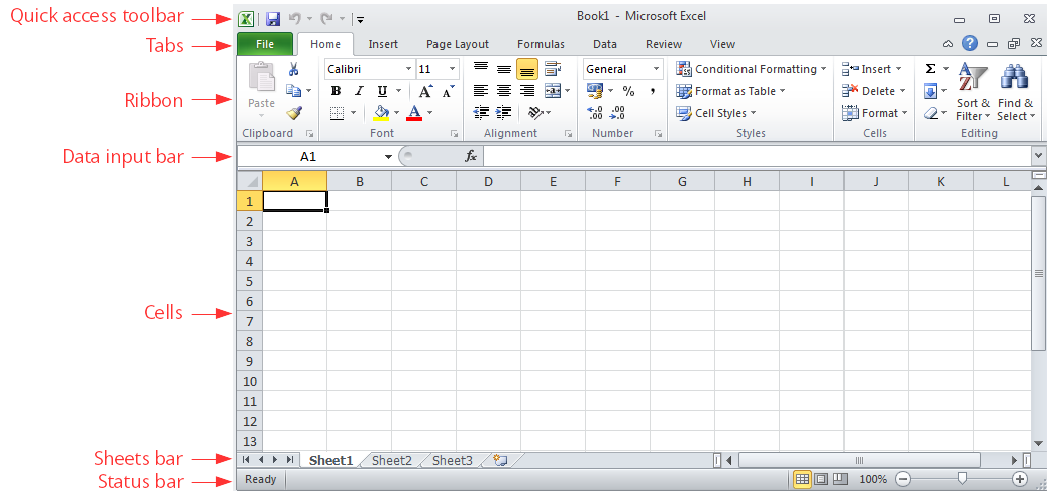
\includegraphics[max width=\linewidth]{../img/excel_2010_screenshot.png}
\end{center}
\caption{Excel 2010 screenshot.}
\label{img-excel_2010_screenshot}
\end{figure}

\section{Excel 2010 ribbon}\hypertarget{excel-2010-ribbon}{}\label{excel-2010-ribbon}

The top ribbon of Excel 2010 contains a lot of buttons that performs different actions. These buttons are arranged in panels, and panels are arranged in tabs. The main ribbon tabs are:

\textbf{File} – Performs file management tasks (new file, open file, save file, print file, etc.). It also contains general configuration options and help.

\begin{center}
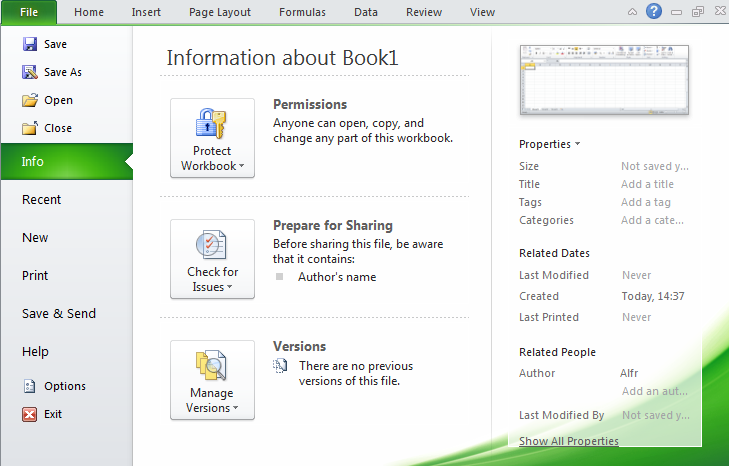
\includegraphics[max width=\linewidth]{../img/excel_2010_file_ribbon.png}
\end{center}

\textbf{Home} – Common tools (clipboard, fonts, alignment, numbers format, insert rows and columns, etc.)

\begin{center}
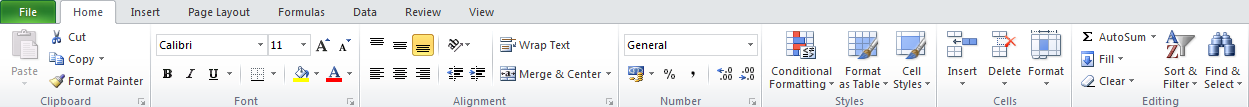
\includegraphics[max width=\linewidth]{../img/excel_2010_home_ribbon.png}
\end{center}

\textbf{Insert} – Insert objects in the sheet (tables, illustrations, charts, hyperlinks, text, equations, etc.)

\begin{center}
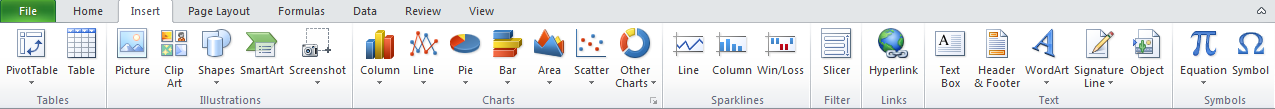
\includegraphics[max width=\linewidth]{../img/excel_2010_insert_ribbon.png}
\end{center}

\textbf{Page Layout} – Configure the printing (page setup, scale, themes, etc. )

\begin{center}
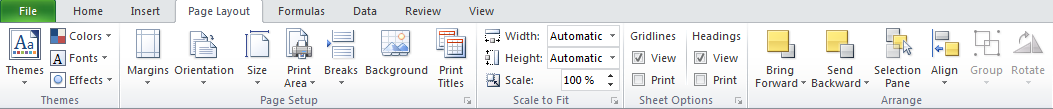
\includegraphics[max width=\linewidth]{../img/excel_2010_page_layout_ribbon.png}
\end{center}

\textbf{Formulas} – Functions arranged in categories and formula auditing.

\begin{center}
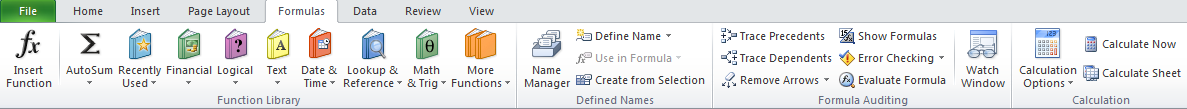
\includegraphics[max width=\linewidth]{../img/excel_2010_formulas_ribbon.png}
\end{center}

\textbf{Data} – Working with databases (import data, connection with databases, sort and filter data, data validation, etc.)

\begin{center}
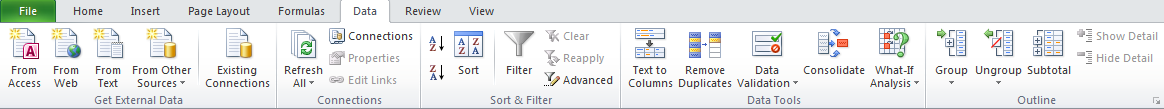
\includegraphics[max width=\linewidth]{../img/excel_2010_data_ribbon.png}
\end{center}

\textbf{Review} – Spelling, commenting, protecting and sharing sheets.

\begin{center}
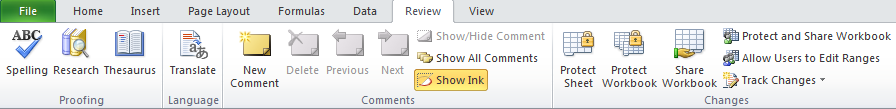
\includegraphics[max width=\linewidth]{../img/excel_2010_review_ribbon.png}
\end{center}

\textbf{View} – How Excel appears on screen (custom windows, grids lines, zoom, windows, etc. Does not affect printing).

\begin{center}
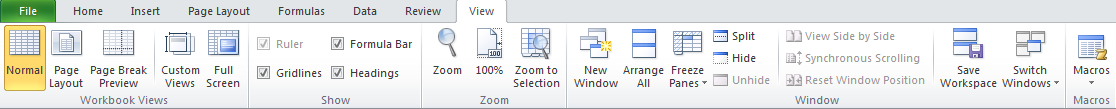
\includegraphics[max width=\linewidth]{../img/excel_2010_view_ribbon.png}
\end{center}


\subsection{Contextual tabs}\hypertarget{contextual-tabs}{}\label{contextual-tabs}

These tabs only appears in some contexts, as for example, when creating a chart or a picture.

\textbf{Chart design} Allows to select the type of chart.

\begin{center}
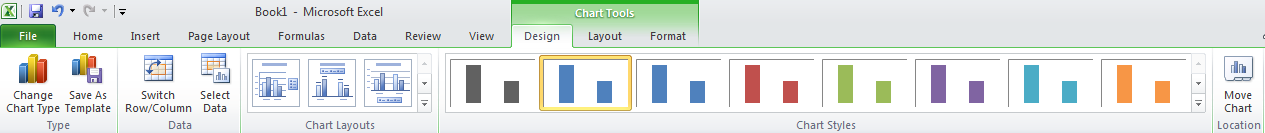
\includegraphics[max width=\linewidth]{../img/excel_2010_design_chart_ribbon.png}
\end{center}

\textbf{Chart layout} Allows to insert and configure some parts of charts (title, axis, leyend, gridlines, etc.)

\begin{center}
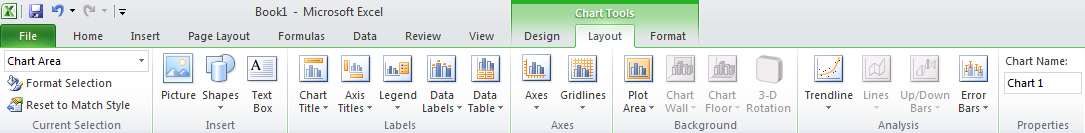
\includegraphics[max width=\linewidth]{../img/excel_2010_layout_chart_ribbon.png}
\end{center}

\textbf{Chart format} Allows to change the aspect of charts (height, width, font, colors, background, etc.)

\begin{center}
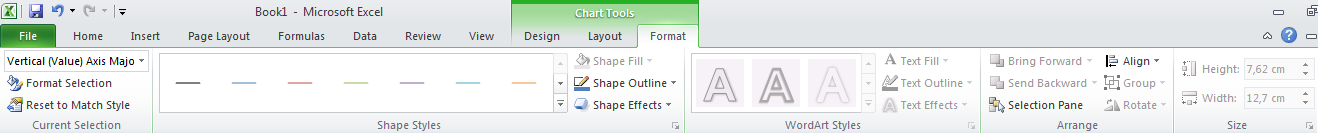
\includegraphics[max width=\linewidth]{../img/excel_2010_format_chart_ribbon.png}
\end{center}

\textbf{Picture} Allows to modify images (borders, rotation, crop, color, filters, special effects, etc.)

\begin{center}
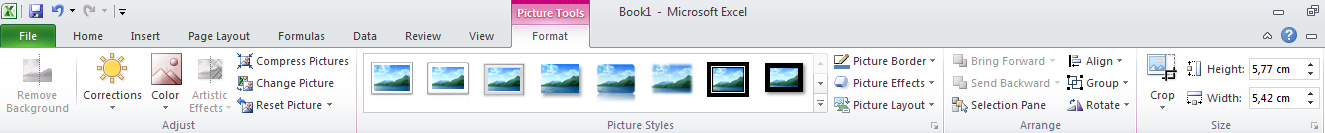
\includegraphics[max width=\linewidth]{../img/excel_2010_picture_ribbon.png}
\end{center}

In addition to these tabs, users can create their own tabs and customise them with buttons as their convenience.

There exists also a quick access toolbar just above the ribbon that can be customised with the most common buttons (see
figure~\ref{img-quick_access_toolbar}.

\begin{figure}[htbp]
\begin{center}
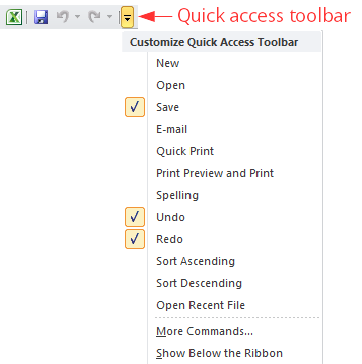
\includegraphics[max width=\linewidth]{../img/quick_access_toolbar.png}
\end{center}
\caption{Excel 2010 quick access toolbar.}
\label{img-quick_access_toolbar}
\end{figure}


\subsection{Access dialogs}\hypertarget{access-dialogs}{}\label{access-dialogs}

When you click the right bottom corner of any panel, the corresponding dialog is show where all the related options are available.

\textbf{Example}. The figure \ref{img-access_font_dialog} shows the font dialog with all the options related to fonts (font family,
font style, font size, etc.)

\begin{figure}[htbp]
\begin{center}
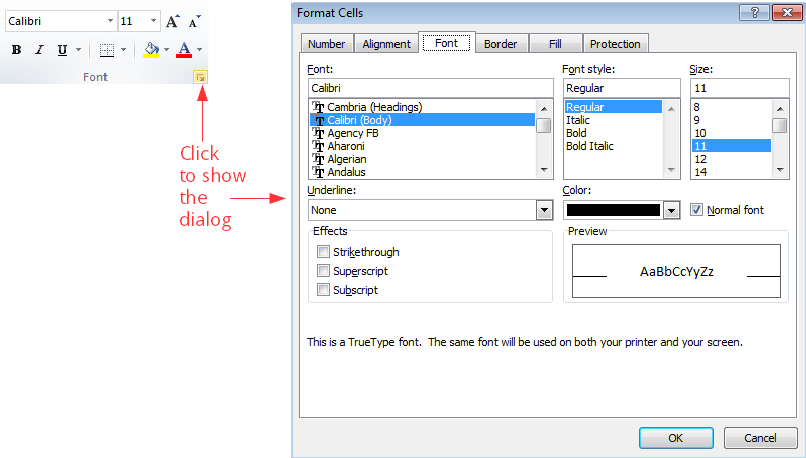
\includegraphics[max width=\linewidth]{../img/access_font_dialog.png}
\end{center}
\caption{Font dialog.}
\label{img-access_font_dialog}
\end{figure}

\subsection{Contextual menu}\hypertarget{contextual-menu}{}\label{contextual-menu}

Clicking the right button of the mouse (right-clicking) a contextual menu is showed with some buttons or options to perform actions in that context. 
This menu has different options depending on the part of the windows that is clicked.

\textbf{Example}. The figure \ref{img-contextual_menu} shows the contextual menu showed right-clicking any cell.

\begin{figure}[htbp]
\begin{center}
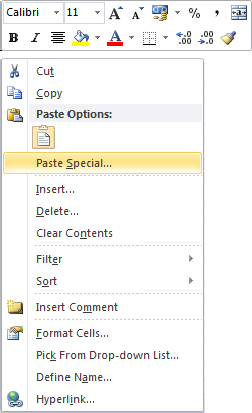
\includegraphics[scale=0.7]{../img/contextual_menu.png}
\end{center}
\caption{Cells contextual menu.}
\label{img-contextual_menu}
\end{figure}

\section{Workbooks, worksheets, rows, columns and cells}\hypertarget{workbooks-worksheets-rows-columns-and-cells}{}\label{workbooks-worksheets-rows-columns-and-cells}

An Excel file is a \emph{workbook} with several \emph{worksheets} that are two dimensional tables divided in \emph{columns} and \emph{rows}. The intersection of a column with a row is a \emph{cell} that is where data are entered. Sheets have a maximum of 16,384 columns and 1,048,576 rows.

Each worksheet has a name and are arranged in tabs at the bottom. Columns and rows have also names; columns are named with letters at the top of the column and rows with numbers to the left of the row. This way each cell is identified by the name of the worksheet, the name of the column and the name of the row where is located, and cells names follow the pattern \texttt{name-of-worksheet ! column-name row-name}. However, to refer to any cell in the active worksheet, the worksheet name may be omitted.

\textbf{Example}. The name of the selected cell in the figure \ref{img-sheet_column_row_cell} is \texttt{Sheet1!C4}.

\begin{figure}[htbp]
\begin{center}
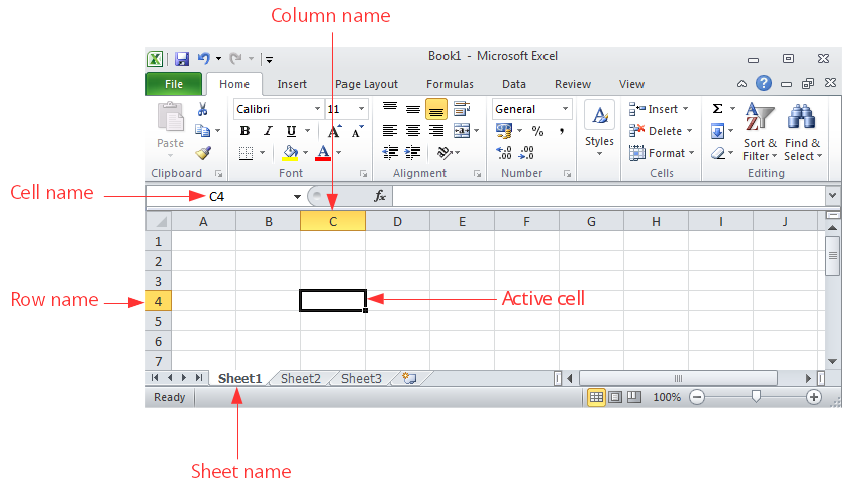
\includegraphics[max width=\linewidth]{../img/sheet_column_row_cell.png}
\end{center}
\caption{Cells, rows, columns and worksheets in Excel.}
\label{img-sheet_column_row_cell}
\end{figure}

The names of rows and columns can not be changed, but worksheet names can be changed double-clicking it and typing the new name.

\subsection{Ranges of cells}\hypertarget{ranges-of-cells}{}\label{ranges-of-cells}

A range of cells is a rectangular block of adjacent cells that is identified by top-left cell and the bottom-right cell separated by a colon, following the pattern \texttt{top-left-cell-name:bottom-right-cell-name}.

\textbf{Example}. In the figure \ref{img-cells_range} the range B3:E5 is selected.

\begin{figure}[htbp]
\begin{center}
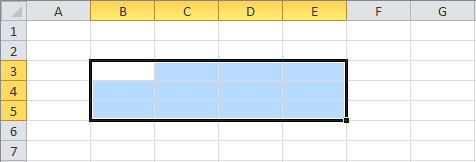
\includegraphics[max width=\linewidth]{../img/cells_range.png}
\end{center}
\caption{Range of cells.}
\label{img-cells_range}
\end{figure}

\subsection{Selecting cells, rows, columns, ranges and worksheets}\hypertarget{selecting-cells-rows-columns-ranges-and-worksheets}{}\label{selecting-cells-rows-columns-ranges-and-worksheets}

To select a cell just click it. 
To select a row click the header of the row or press the keys \texttt{Shift+Spacebar}. 
To select a column click the header of the column or press the keys \texttt{Ctrl+Spacebar}.
To select a range click one corner cell and drag the cursor over the desired cells. 
To select the whole worksheet click the top-left corner of the worksheet o press the keys \texttt{Ctrl+A}.

\textbf{Example}.  This \href{http://aprendeconalf.es/office/excel/manual/img/example_cells_selection.gif}{animation} shows how to select the cell C3, after the row 3, after the column C, after range B3:D7 and finally the whole worksheet.

\section{Data edition}\hypertarget{data-edition}{}\label{data-edition}

\subsection{Insert data}\hypertarget{insert-data}{}\label{insert-data}

Data are entered into the cells activating the cell (clicking it) and typing directly in the cell or in the input bar.

\textbf{Example}.  This \href{http://aprendeconalf.es/office/excel/manual/img/example_enter_data.gif}{animation} shows how to enter the text `Excel' in cell B2 and the number 2010 in cell C2, and after change the number of cell C2 to 2013.

Excel has a smart autocomplete feature that proposes completing the data that is typed with some predictions.

\subsection{Delete data}\hypertarget{delete-data}{}\label{delete-data}

To delete the content of a cell or a range of cells simply select the it and press \texttt{Supr} key. It's also possible to delete the cell contents with the button \texttt{Clear All}.

\subsection{Remove cells, rows, columns and worksheets}\hypertarget{remove-cells-rows-columns-and-worksheets}{}\label{remove-cells-rows-columns-and-worksheets}

To remove a whole cell (no only the content), right-click the cell and select the option \texttt{Delete...}. In the dialog that appears select \texttt{Shift cells left} if you want the cells to the left of the removed cell move to the left to fill the gap, or \texttt{Shift cells up} if you want the cells below the removed cell move up to fill the gap.

To remove a whole row, right-click the header of the row and select the option  \texttt{Delete...}.

To remove a whole column, right-click the header of the column and select the option  \texttt{Delete...}.

To remove a worksheet, right-click the tab with the name of the worksheet and select the option \texttt{Delete...}. 
\emph{Warning: Removing worksheets can not be undone!}

\textbf{Example}.  This \href{http://aprendeconalf.es/office/excel/manual/img/example_data_remove.gif}{animation} shows how to remove a cell, a row, a column and a worksheet.

\subsection{Insert cells, rows, columns and worksheets}\hypertarget{insert-cells-rows-columns-and-worksheets}{}\label{insert-cells-rows-columns-and-worksheets}

To insert a new cell in a position, right-click the current cell in that position and select the option \texttt{Insert...}.  In the dialog that appears select \texttt{Shift cells right} if you want to move the cells to the right to make a gap for the new cell, or \texttt{Shift cells down} if you want to move the cells down to make a gap for the new cell.

To insert a new row, right-click the header of the row above which you want to insert the new row and select \texttt{Insert}.

To insert a new column, right-click the header of the column to the left of which you want to insert the new column and select \texttt{Insert}.

To insert a new worksheet, right-click the tab with the name of the worksheet to the left of which you want to insert the new worksheet and select \texttt{Insert}.
In the dialog that appears select `Worksheet'.

\textbf{Example}.  This \href{http://aprendeconalf.es/office/excel/manual/img/example_data_insert.gif}{animation} shows how to insert a cell, a row, a column and a worksheet.

\subsection{Cut, copy and paste}\hypertarget{cut-copy-and-paste}{}\label{cut-copy-and-paste}

Like in many other Windows applications, you can use the clipboard to cut, copy and paste cells, rows, columns and ranges contents.

To cut or copy a cell, row, column or range, right-click it and select the option \texttt{Cut} or \texttt{Copy} respectively, or press the keys \texttt{Ctrl+x} or \texttt{Ctrl+c} respectively. Both options copy the content of the cell, row, column or range to the clipboard, but the difference between cut and copy is that cut delete the content from the current cell, row, column or range, while copy no.

To paste the content of the clipboard in a new cell, row, column or range, select the cell or the first cell of the row, column or range and click the button \texttt{Paste} or press the keys \texttt{Ctrl+v}.

\textbf{Example}.  This \href{http://aprendeconalf.es/office/excel/manual/img/example_copy_paste.gif}{animation} shows how to copy and paste the content of a cell, a row, a column and a range and a worksheet.

\subsection{Autofill}\hypertarget{autofill}{}\label{autofill}

An useful feature of Excel is the autofill of cells following a serie or pattern. In some cases, like for example dates, it is enough to write the content of the first cell and then click the bottom-right corner of the cell and drag the cursor over the column or row to get the cells filled with the following dates.

For number or text, this actions replicates the content of the first cell in the others. To autofill with a serie of numbers is necessary to enter the first two numbers of the serie in two consecutive cells, then select both cells, click the bottom-left corner and drag the cursor over the column or row to get the cells filled with the numbers following the serie.

\textbf{Example}. This \href{http://aprendeconalf.es/office/excel/manual/img/example_autofill.gif}{animation} shows how
to replicate the content of cell A1 to range A2:A10, next how to auto fill the range B1:B10 with the following dates to the date in cell B1, and finally how to auto fill the range C1:C10 with the serie of even numbers.


\subsection{Undo and redo}\hypertarget{undo-and-redo}{}\label{undo-and-redo}

In the quick access toolbar there are buttons \texttt{Undo} 
\includegraphics[max width=\linewidth]{../img/button_undo.png} and \texttt{Redo} 
\includegraphics[max width=\linewidth]{../img/button_redo.png}. The \texttt{Undo} button undoes the last data edition action performed and the \texttt{Redo} button reverses the last undone action. If you press the undo button several $n$ times, it undoes the last $n$ actions, and the same happens with the redo button.

\textbf{Example}.  This \href{http://aprendeconalf.es/office/excel/manual/img/example_undo.gif}{animation} shows how to remove the content of cell B2, then change the content of cell C2 two times, then undo that actions and finally redo the same actions.

\section{Column and row sizing}\hypertarget{column-and-row-sizing}{}\label{column-and-row-sizing}

Columns width and rows height can be easily changed. To change the width of a column click the line between the column you want to resize and the next column in the column header, and then drag the pointer mouse to increase or reduce the column width. If you double-click this line the column width will auto resize to the width of the widest cell content in the column.

In a similar way, to change the height of a row click the line between the row you want to resize and the next row in the row header, and then drag the pointer mouse to increase or reduce the row height. If you double-click this line the row height will auto resize to the height of the highest cell content in the row.

\textbf{Example}.  This \href{http://aprendeconalf.es/office/excel/manual/img/example_row_column_resize.gif}{animation} shows how to resize the width of column C and the height of row 3 to fit the content of cell C3.

% <!--
% ![row and column sizing.](img/row_column_sizing.png "row and column sizing")
% </div> 
% -->

\section{File management}\hypertarget{file-management}{}\label{file-management}

Data of workbooks are stored in files. Although Excel makes backups copies of your work regularly, is a good practice to save your work in files often.

\subsection{Save a file}\hypertarget{save-a-file}{}\label{save-a-file}

To save the content of a workbook in a file press the tab \texttt{File} and select the option \texttt{Save}. In the dialog that appears type the file name and select the storage unit and folder where to save the file. The default extension for Excel 2010 file names is \emph{xlsx}.

\subsection{Open a file}\hypertarget{open-a-file}{}\label{open-a-file}

To open an Excel file press the tab \texttt{File} and select the option \texttt{Open}.
In the dialog that appears select the storage unit and folder where the file is saved and the file to open, an press the button \texttt{Open}.

\subsection{Create a new workbook}\hypertarget{create-a-new-workbook}{}\label{create-a-new-workbook}

To create a new workbook press the tab \texttt{File} and select the option \texttt{New}. In the dialog that appears select \texttt{Blank workbook}. It's possible to create new workbooks from predefined templates.

\subsection{Close a workbook}\hypertarget{close-a-workbook}{}\label{close-a-workbook}

To close an open workbook press the tab \texttt{File} and select the option \texttt{Close}. If the last changes in the workbook haven't been saved, a warning will appear allowing you to save the file before to close it.

\section{Exporting and importing data}\hypertarget{exporting-and-importing-data}{}\label{exporting-and-importing-data}

Excel can export and import data in many formats. One of the most common formats is csv (comma separated values). In this format data is saved in a plain text file one row per line and separating columns with commas or semicolons.

\subsection{Export to csv format}\hypertarget{export-to-csv-format}{}\label{export-to-csv-format}

To export a worksheet to csv format file, click the option \texttt{Save as} of the ribbon's \texttt{File} tab. In the dialog that appears select the option \texttt{CSV (Comma delimited) (*.csv)} from the drop-down list \texttt{Save as type}, give a name to the file, select the folder where to save it and click OK.

\textbf{Example}. This \href{http://aprendeconalf.es/office/excel/manual/img/example_export_csv.gif}{animation} shows
how to export a worksheet with a students database to a csv format file.


\subsection{Import from csv format}\hypertarget{import-from-csv-format}{}\label{import-from-csv-format}

To import csv format file click the option \texttt{Open} of the ribbon's \texttt{File} tab. In the dialog that appears click the button to the right of the File name box and select the option \texttt{Text Files (*.prn;*.txt;*.csv)}, select the csv format file and click OK.

If you want more control in the importation process, click the \texttt{From Tex} button of the \texttt{Get External Data} in the ribbon's \texttt{Data} tab. In the dialog that appears select the csv format file and click the \texttt{Import} button. This brings another dialog where you can select if fields are delimited by a special character or are a fixed number of characters, the delimiter character (Tab, Semicolon, Comma, Space or other), the data format or every column (General, Text or Date). After that click the \texttt{Finish} button and in the dialog that appears select the cell where to put the imported data and click OK.

\textbf{Example}. This \href{http://aprendeconalf.es/office/excel/manual/img/example_import_csv.gif}{animation}
shows how to import the csv format file with the students database of the previous example.


\section{Getting help}\hypertarget{getting-help}{}\label{getting-help} 

One of the most useful features of Microsoft Office programs is the system of help that they have. To get help about any issue in Excel click the option \texttt{Help} in the Help tab of the ribbon, and then click \texttt{Microsoft Office Help}. This shows a browser where you can enter some key words and Excel will search topics related to these words and present the search results in a list. Clicking the desired topic will show you help info about that topic.

\textbf{Example}. The figure \ref{img-excel_2010_help} shows the help search results for the word ``cell''.

\begin{figure}[htbp]
\begin{center}
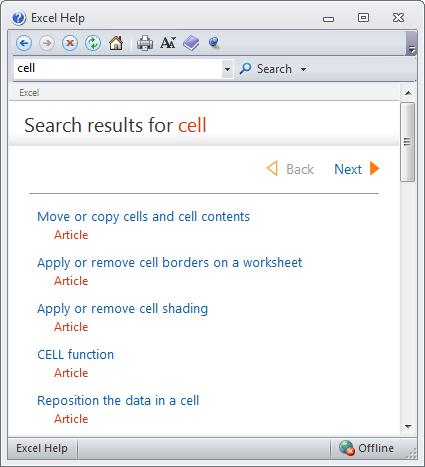
\includegraphics[scale=0.7]{../img/excel_2010_help.png}
\end{center}
\caption{Excel 2010 help.}
\label{img-excel_2010_help}
\end{figure}

 
% Autor: Alfredo Sánchez Alberca (email:asalber@ceu.es)

\chapter{Formatting data}

Content of cells can be formatted in many ways: changing the data type, the font family, the alignment, the color, the border, etc. Most formatting options are grouped in the \emph{Format Cells} dialog. To show this dialog click the bottom right corner of the Font panel in the ribbon's Home tab.

\section{Data types}\hypertarget{data-types}{}\label{data-types}

Excel manages several data types. The most common are numbers, dates and times, and text. All available data types are
in the \texttt{Number tab} of the Format Cells dialog (see figure~\ref{img-number_dialog}).

\begin{figure}[htbp]
\begin{center}
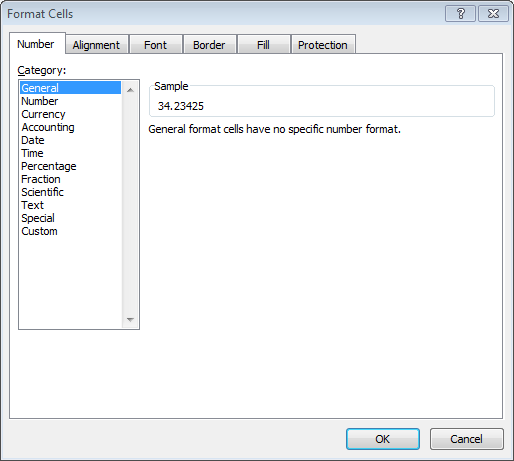
\includegraphics[scale=0.7]{../img/number_dialog.png}
\end{center}
\caption{Number dialog.}
\label{img-number_dialog}
\end{figure}

\subsection{Formatting numbers}\hypertarget{formatting-numbers}{}\label{formatting-numbers}

By default cells with numeric content are of type \emph{Number}, but there are other numeric types like \emph{Currency}
and \emph{Accounting}. Number is used for general display of numbers, while Currency and Accounting are used for
monetary values. In all cases you can specify the number of decimal places. For monetary values you can also specify the
symbol for the currency (\euro\ by default).

\textbf{Example}. The table in this \href{http://aprendeconalf.es/office/excel/manual/img/example_number_format.gif}{animation} shows the price of fruits during several months and the average price. The animation shows how to change the format of prices to currency type with 3 decimal places.

\subsection{Formatting dates and times}\hypertarget{formatting-dates-and-times}{}\label{formatting-dates-and-times}

By default cells with content following the pattern \texttt{day/month/year} are of type \emph{Date}, but there are a lot of ways of formatting dates, like for example, \texttt{year-month-day} or \texttt{day-month\_name-year} etc.

\textbf{Example}. The table in this \href{http://aprendeconalf.es/office/excel/manual/img/example_date_format.gif}{animation} shows the price of fruits during several months and the average price. The animation shows how to change the format of dates following the pattern Month-Year, with the three first letters of months and the two last digits of years.

By default cells with content following the pattern \texttt{hours:minutes:seconds} are of type \emph{Time}, but there are a several ways of formatting times.

\subsection{Formatting text}\hypertarget{formatting-text}{}\label{formatting-text}

By default cells with non numeric content are of type \emph{Text}. It's possible to apply this type even to numbers, like for example phone numbers.

Text entered in a cell spreads to adjacent cells to the right if these cells have no content. To confine text to a certain width in the cell, select the cell and click the button \texttt{Wrap Text} in the Alignment section in the ribbon's Home tab.

\section{Align cell contents}\hypertarget{align-cell-contents}{}\label{align-cell-contents}

By default numbers are aligned to the right and text to the left, but it's possible to change the alignment of cell
contents in the \texttt{Alignment tab} of the Format Cells dialog (see figure~\ref{img-alignment_dialog}).

\begin{figure}[htbp]
\begin{center}
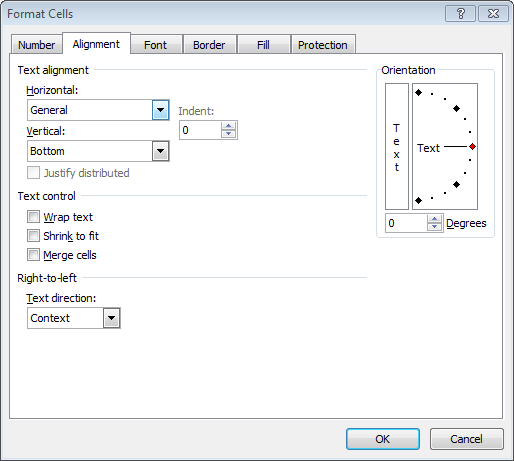
\includegraphics[scale=0.7]{../img/alignment_dialog.png}
\end{center}
\caption{Alignment dialog.}
\label{img-alignment_dialog}
\end{figure}

\subsection{Horizontal alignment}\hypertarget{horizontal-alignment}{}\label{horizontal-alignment}

To change the horizontal alignment select Left, Right, Center or Justify in the Horizontal drop down list of the
\texttt{Alignment tab}. You can also align the cell contents with the buttons of the Alignment panel in the Home tab of
the ribbon (see figure~\ref{img-button_horizontal_alignment}).

\begin{figure}[htbp]
\begin{center}
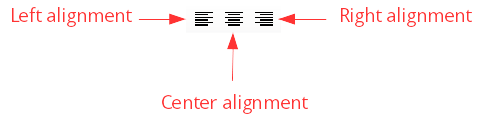
\includegraphics[scale=0.7]{../img/button_horizontal_alignment.png}
\end{center}
\caption{Horizontal alignment buttons.}
\label{img-button_horizontal_alignment}
\end{figure}

\textbf{Example}. The table in this \href{http://aprendeconalf.es/office/excel/manual/img/example_alignment.gif}{animation} shows the price of fruits during several months and the average price. The animation shows how to align the average prices centered.

\subsection{Vertical alignment}\hypertarget{vertical-alignment}{}\label{vertical-alignment}

To change the vertical alignment select Top, Bottom, Center or Justify in the Vertical drop down list of the
\texttt{Alignment tab}. You can also align the cell contents with the buttons of the Alignment panel in the Home tab of
the ribbon (see figure~\ref{img-button_vertical_alignment}).

\begin{figure}[htbp]
\begin{center}
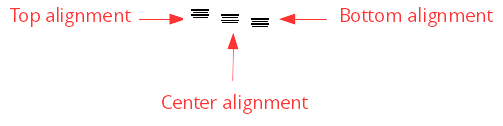
\includegraphics[scale=0.7]{../img/button_vertical_alignment.png}
\end{center}
\caption{Vertical alignment buttons.}
\label{img-button_vertical_alignment}
\end{figure}

\section{Font properties}\hypertarget{font-properties}{}\label{font-properties}

To format the font of cell contents select the font family, font style, font size and font color from the \texttt{Font
tab} of the Format Cells dialog (see figure~\ref{img-font_dialog}). You can also apply some effects like underline, superscript
and subscript.

\begin{figure}[htbp]
\begin{center}
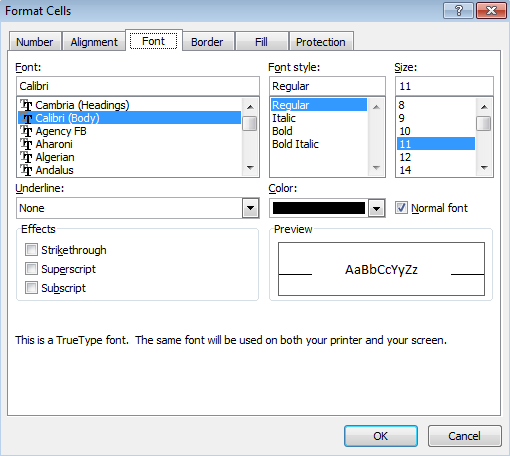
\includegraphics[scale=0.7]{../img/font_dialog.png}
\end{center}
\caption{Font dialog.}
\label{img-font_dialog}
\end{figure}

It's also possible to change the font family, style, size and color from the Font panel in the ribbon's Home tab, and also with the contextual toolbar that appears right-clicking the cell.

\textbf{Example}. The table in this
\href{http://aprendeconalf.es/office/excel/manual/img/example_font_family.gif}{animation} shows the price of fruits
during several months and the average price. The animation shows how to change the font family of all table to Arial,
size 10 pt. 

And this \href{http://aprendeconalf.es/office/excel/manual/img/example_font_colour.gif}{animation} also shows how
to change the font style of average prices to bold and the color of fruits names to blue.


\section{Borders and background}\hypertarget{borders-and-background}{}\label{borders-and-background}

To format the borders of cells select the line style and color, and click the borders where to apply that line in the
table of the \texttt{Borders tab} in the Format Cells dialog (see figure~\ref{img-border_dialog}).

\begin{figure}[htbp]
\begin{center}
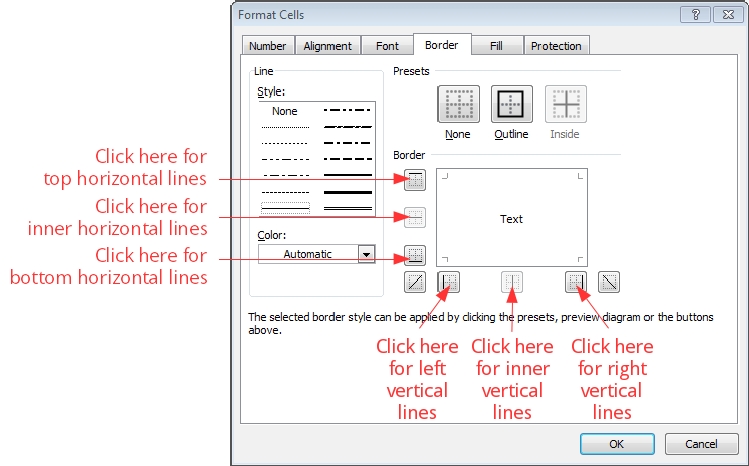
\includegraphics[scale=0.7]{../img/border_dialog.png}
\end{center}
\caption{Border dialog.}
\label{img-border_dialog}
\end{figure}

It's also possible to change the border of cells with the \texttt{Border button}

\includegraphics[scale=0.7]{../img/button_border.png} of the Font panel in the ribbon's Home tab, and also with the
contextual toolbar that appears right-clicking the cell.

\textbf{Example}. The table in this
\href{http://aprendeconalf.es/office/excel/manual/img/example_borders.gif}{animation} shows the price of fruits during several months and the average price. The animation shows how to put lines to some cell borders.

To format the background of cells select the background color and pattern style in the \texttt{Fill tab} of the Format
Cells dialog (see figure~\ref{img-fill_dialog}).

\begin{figure}[htbp]
\begin{center}
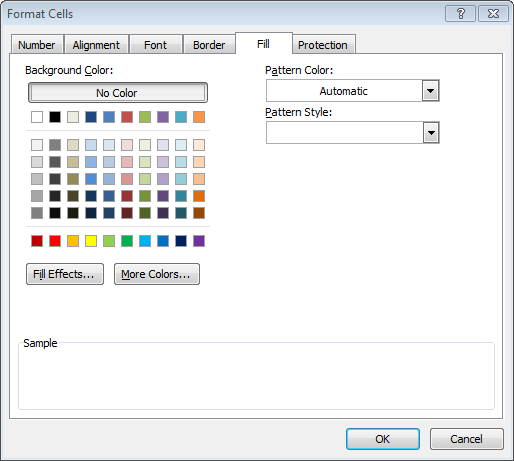
\includegraphics[scale=0.7]{../img/fill_dialog.png}
\end{center}
\caption{Fill dialog.}
\label{img-fill_dialog}
\end{figure}

It's also possible to change the background color of cells with the \texttt{Background colour} button 

\includegraphics[scale=0.7]{../img/button_background_colour.png} of the Font panel in the ribbon's Home tab, and
also with the contextual toolbar that appears right-clicking the cell.

\textbf{Example}. The table in this \href{http://aprendeconalf.es/office/excel/manual/img/example_background_colour.gif}{animation} shows the price of fruits during several months and the average price. The animation shows how set the background colour of some cells.

\section{Merge cells}\hypertarget{merge-cells}{}\label{merge-cells}

To merge several cells in one, select the range of cells and click the button \texttt{Merge \& Center} in the Alignment
section in the ribbon's Home tab. If there are more than one cell with content in the range, merging will keep the
content of the upper-left cell only. By default content of merged cells is centered.

\textbf{Example}. The table in this \href{http://aprendeconalf.es/office/excel/manual/img/example_merge_cells.gif}{animation} shows the price of fruits during several months and the average price. The animation shows how merge the cells of the first row and center the title.

\section{Copy and paste format}\hypertarget{copy-and-paste-format}{}\label{copy-and-paste-format}

To apply the format of a cell to others select the cell, click the \texttt{Format painter} button 

\includegraphics[scale=0.7]{../img/button_format_painter.png} to copy the cell format. Then then select the range of
cells to paste the that format.

\textbf{Example}. The table in this \href{http://aprendeconalf.es/office/excel/manual/img/example_format_painter.gif}{animation} shows the price of fruits during several months and the average price. The animation shows how to apply the same format of the fruit rows to a new row for pineapples.

\section{Conditional formatting}\hypertarget{conditional-formatting}{}\label{conditional-formatting}

Excel allows to apply a format to a cell depending according to some rules. To set a new rule click the \texttt{Conditional Formatting} button and select \texttt{New Rule}. There are different types of rules:

\begin{itemize}
\item \textbf{Format all cells based on their value} Applies a format style based on the value of the cell. There are 4 types of styles:


\begin{itemize}
\item \emph{2-Color Scale} Applies a colour in a continuous scale ranging from one colour for the minimum value or percentage to other colour for the maximum value or percentage.

\textbf{Example}. The table in this \href{http://aprendeconalf.es/office/excel/manual/img/example_conditional_formatting_colour_scale.gif}{animation} shows the price of fruits during several months and the average price. The animation shows how to apply to prices a colour background in a continuous scale from green (the minimum price) to red (the maximum price).
\item \emph{3-Color Scale} The same than 2-Color Scale but with a third intermediate colour in the scale.
\item \emph{Data bar} Plots an horizontal bar in each cell with a with proportional to the value of the cell.

\textbf{Example}. The table in this \href{http://aprendeconalf.es/office/excel/manual/img/example_conditional_formatting_data_bar.gif}{animation} shows the price of fruits during several months and the average price. The animation shows how to apply to prices a data bar format.
\item \emph{Icon Sets} Divide the distribution of selected cell values in several parts according to intervals or percentiles, assign an different icon to each part, and plot the corresponding icon in each cell.

\textbf{Example}. The table in this \href{http://aprendeconalf.es/office/excel/manual/img/example_conditional_formatting_icon_set.gif}{animation} shows the price of fruits during several months and the average price. The animation shows how to apply to prices an icon set format. The icon set has three icons: red is applied to values under the 33 percentile, yellow is applied to values between 33 and 67 percentiles, and green is applied to values over 67 percentile.
\end{itemize}
\item \textbf{Format only cells that contain} Applies a format to the cell if satisfies a logical condition.
\end{itemize}

\textbf{Example}. The table in this \href{http://aprendeconalf.es/office/excel/manual/img/example_conditional_formatting_logical_condition.gif}{animation} shows the price of fruits during several months and the average price. The animation shows how to apply to prices higher than 2 € a red colour.

\begin{itemize}
\item \textbf{Format only top or bottom ranked values} Applies a format to a number or percentage of top or bottom values.
\end{itemize}

\textbf{Example}. The table in this \href{http://aprendeconalf.es/office/excel/manual/img/example_conditional_formatting_top_values.gif}{animation} shows the price of fruits during several months and the average price. The animation shows how to apply to the three top higher prices a red colour.

\begin{itemize}
\item \textbf{Format only values that are above or below average} Applies a format to cells with values above or below the average of selected cells.
\end{itemize}

\textbf{Example}. The table in this \href{http://aprendeconalf.es/office/excel/manual/img/example_conditional_formatting_average.gif}{animation} shows the price of fruits during several months and the average price. The animation shows how to apply a red colour to prices above the average and a green colour to prices below the average.

\section{Predefined styles}\hypertarget{predefined-styles}{}\label{predefined-styles}

Excel has a lot of predefined styles for formatting cells and tables. To apply a predefined cell style click
\texttt{Cell Styles} button and select the desired style. It's possible to define new cell styles. For that select the
cell with the format to define as a style, click \texttt{Cell Styles} button and select \texttt{New Cell Style}
option. In the dialog that appears just give a name to the new style, press OK, and the new cell style will appear in
the cell styles menu.

To apply a predefined table style click \texttt{Format as Table} button and select the desired style. It's also possible
to define new table styles. For that click \texttt{Format as Table} button and select \texttt{New Table Style} option.
In the dialog that appears just give a name to the new style, define the table format (font, borders and fill), press OK,
and the new table style will appear in the table styles menu.

 
% Autor: Alfredo Sánchez Alberca (email:asalber@ceu.es)

\chapter{Calculus with formulas}

Spreadsheets are used mainly for doing calculations and one of the most powerful features of spreadsheets are
calculation formulas. In this section we will see how to use them.

\section{Enter formulas}\hypertarget{enter-formulas}{}\label{enter-formulas}

To enter a formula in a cell always start typing an equal sign \texttt{=} and then the formula expression.

Formula expressions can contain arithmetic operators: addition \texttt{+}, subtraction \texttt{-}, multiplication
\texttt{*}, division \texttt{/} and powers \texttt{\^{}} and named predefined functions like \texttt{SUM}, \texttt{EXP},
\texttt{SIN}, etc. This allow to use Excel as a calculator. When Excel evaluates expressions first evaluate named
functions, then powers, then products and quotients, and finally additions and subtractions, but it's possible to use
parenthesis to force the evaluation of a subexpression before.

\textbf{Example} Assuming that cells A1, B1 and C1 contain the values 6, 3 and 2 respectively, the next table shows some
formulas and their respective results.

\begin{longtable}{cc}
\toprule
Formula & Result\\
\midrule
\endfirsthead
A1+B1-C1 & 7\\
A1+B1*C1 & 12\\
(A1+B1)*C1 & 18\\
A1/B1-C1 & 0\\
A1/(B1-C1) & 6\\
A1+B1\^{}C1 & 15\\
(A1+B1)\^{}C1 & 81\\
\bottomrule
\end{longtable}



\textbf{Example}. This \href{http://aprendeconalf.es/office/excel/manual/img/example_enter_formulas.gif}{animation} shows how to enter the formula 4+2 in cell A1, the formula 4-2 in cell B1, the formula 4*2 in cell C1, the formula 4/2 in cell D1, the formula 4\^{}2 in cell E1 and the formula ((4+1)*2)\^{}3 in cell F1.

\section{Using relative and absolutes cell references in formulas}\hypertarget{using-relative-and-absolutes-cell-references-in-formulas}{}\label{using-relative-and-absolutes-cell-references-in-formulas}

Formula expressions can content references to cells. When Excel evaluates formulas it replace every cell reference by its content before doing the calculation.

\textbf{Example}. This
\href{http://aprendeconalf.es/office/excel/manual/img/example_formulas_with_references.gif}{animation} shows how to use
the formula \texttt{=A1+B1} to add up the content of cells A1 and B1 in cell C1.

References that are formed by the name of the cell or range are known as \emph{relative references}, because referenced
cells change when you copy a cell with a formula and paste in another cell. In general, when you copy a formula $n$
columns to the right and $m$ rows down, the referenced cells in the formulas will be updated by the cells $n$ columns to
the right and $m$ rows down, an the same if you copy the cell to the left or top.

\textbf{Example}. This \href{http://aprendeconalf.es/office/excel/manual/img/example_copying_formulas_with_relative_references.gif}{animation} shows how to copy the formula \texttt{=A1+B1} in cell C1, with relative references to A1 and B1, to the cell E4, that is 2 columns to the right and 3 rows down. Observe how the formula in cell E4 is updated to \texttt{=C4+D4}.

A common way of copying the formula of a cell to adjacent cells is clicking the bottom-right corner of the cell and
dragging the cursor to the desired range of cells.

\textbf{Example}. This \href{http://aprendeconalf.es/office/excel/manual/img/example_fibonacci_serie.gif}{animation}
shows how to generate the first ten numbers of the Fibonacci sequence. Cells A1 and B1 contains the two first numbers of
the serie and cell C1 the formula \texttt{=A1+B1} that add the two first numbers up and gives the third number of the
serie. For generating the rest of the serie it is enough to copy the formula of cell C1 to the range D1:J1. Observe how
references in formulas of these cells are updated.

Although relative references are very helpful in many cases, sometimes we need the references in a formula to remain
fixed when copied elsewhere.
In that case we need to use \emph{absolute references}, that are like relative references but preceding the column name
or the row name with a \$ sign to fix either the row, the column or both on any cell reference.

\textbf{Example}. This
\href{http://aprendeconalf.es/office/excel/manual/img/example_copying_formulas_with_absolute_references.gif}{animation} shows how to calculate the IVA of a list of prices. Cells A2 to A5 contains the prices and cell F1 contains the IVA percentage. For calculating the IVA of first price we use the formula \texttt{A2*F\$4/100} where we fix the row of cell F4 because we wan it remain fixed when copying the formula down. Observe how the reference to cell F4 doesn't change when copying the formula down.

\textbf{Example}. This
\href{http://aprendeconalf.es/office/excel/manual/img/example_multiplication_table.gif}{animation} shows how to
calculate the multiplication table using absolute references.

In general, if you want to fix a reference in a formula that you pretend to copy horizontally, you must precede the
column name with a \$ sign; and if you pretend to copy the formula vertically, you must precede the row name with a \$
sign. 

\subsection{Naming cells and ranges}\hypertarget{naming-cells-and-ranges}{}\label{naming-cells-and-ranges}

Cell references are somewhat abstract, and don't really communicate anything about the data they contain. This makes
formulas that involve multiple references difficult to understand. To overcome this difficulty Excel allows to give name
to cells or ranges. To define a cell or range name, select or cell range and click the \texttt{Define Name} button of
the \texttt{Defined Names} panel in the ribbon's \texttt{Formulas} tab. In the dialog that appears give a
name to the cell and click OK. Cell or range names must begin with a letter and can't include spaces.

You can also set the name of a cell or range in the name box of the input bar (see figure~\ref{img-name_box}).

\begin{figure}[htbp]
\begin{center}

\includegraphics[scale=0.7]{../img/name_box.png}
\end{center}
\caption{Name box for giving names to cells or ranges.}
\label{img-name_box}
\end{figure}

After that you can use that cell o range name in any formula. Observe that references with names are always absolutes.

\textbf{Example}. This \href{http://aprendeconalf.es/office/excel/manual/img/example_formulas_with_defined_names.gif}{animation} shows how to calculate the IVA of a list of prices using a cell name for the cell that contains the IVA percentage.

\section{Basic functions}\hypertarget{basic-functions}{}\label{basic-functions}

Excel has a huge library of predefined functions that performs different calculations organised by categories. There are three ways to to enter a function in a formula expression:

\begin{itemize}
\item Type it rawly if you know its name and syntax.
\item Select it from the buttons of the \texttt{Functions Library} panel in the ribbon's \texttt{Formulas} tab.
\end{itemize}

\begin{center}
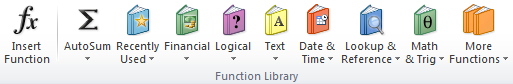
\includegraphics[scale=0.7]{../img/panel_formulas.png}
\end{center}

\begin{itemize}
\item Click the \texttt{Insert Function} button 
\includegraphics[scale=0.7]{../img/button_insert_function.png} from the
input bar.
This will show you a dialog where you can type some key words for looking the desired function an select it (see
figure~\ref{img-dialog_insert_function}).
This dialog also shows help about the function and its syntax.
\end{itemize}

\begin{figure}[htbp]
\begin{center}
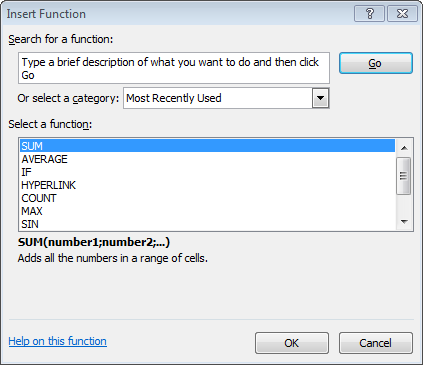
\includegraphics[scale=0.7]{../img/dialog_insert_function.png}
\end{center}
\caption{Insert function dialog.}
\label{img-dialog_insert_function}
\end{figure}

\subsection{SUM function}\hypertarget{sum-function}{}\label{sum-function}

The most common function is \texttt{SUM} that calculates the sum of several numbers. Its syntax is
\texttt{SUM(number1,number2,...)} where \emph{number1, number2}, etc. are the numbers or cell ranges that you want to
sum.

\textbf{Example} This \href{http://aprendeconalf.es/office/excel/manual/img/example_function_sum.gif}{animation} shows how to calculate the sum of the subject grades for every student in a course.

\subsection{SUMIF function}\hypertarget{sumif-function}{}\label{sumif-function}

The \texttt{SUMIF} function its similar to the \texttt{SUM} function but only sum numbers that satisfied a given
criterion.
Its syntax is \texttt{SUMIF(range,criterion,sum-range)} \emph{range} is the cell range to check the criterion,
\emph{criterion} is the condition expression of the criterion, \emph{sum-range} is the range with the values to sum (if
this argument is not provided, the sum is calculated over the values of the \emph{range} argument that meet the
criterion).

The expression with the condition can be a number, a cell reference, a logical expression starting with a logical
operator
(\texttt{=},\texttt{\textgreater{}},\texttt{\textless{}},\texttt{\textgreater{}=},\texttt{\textless{}=},\texttt{\textless{}\textgreater{}})
in double quotes, or a pattern text with wildcards like the question mark \texttt{?} (that matches any
character) or the asterisk \texttt{*} (that matches any character string) in double quotes. 

\textbf{Example} This \href{http://aprendeconalf.es/office/excel/manual/img/example_function_sumif.gif}{animation} shows how to calculate the sum of the grades greater than or equal to 5 for every student in a course.

\subsection{COUNT function}\hypertarget{count-function}{}\label{count-function}

The \texttt{COUNT} function counts the number of cells with numbers in a range.  Its syntax is
\texttt{COUNT(value1,value2,...)} where \emph{value1, value2}, etc. are the values or cell ranges to count.

\textbf{Example} This \href{http://aprendeconalf.es/office/excel/manual/img/example_function_count.gif}{animation} shows how to calculate the number of subjects grades for every student in a course.

\subsection{COUNTIF function}\hypertarget{countif-function}{}\label{countif-function}

The \texttt{COUNTIF} function its similar to the \texttt{COUNT} but only counts number of cells that satisfied a given criterion. Its syntax is \texttt{SUMIF(range,criterion)} \emph{range} is the cell range to check the criterion and \emph{criterion} is the condition expression of the criterion,.

The expression with the condition can be a number, a cell reference, a logical expression starting with a logical
operator
(\texttt{=},\texttt{\textgreater{}},\texttt{\textless{}},\texttt{\textgreater{}=},\texttt{\textless{}=},\texttt{\textless{}\textgreater{}})
in double quotes, or a pattern text with wildcards like the question mark \texttt{?} (that matches any character)
or the asterisk \texttt{*} (that matches any character string) in double quotes.

\textbf{Example} This \href{http://aprendeconalf.es/office/excel/manual/img/example_function_countif.gif}{animation} shows how to calculate the number of passed subjects (grade greater than or equal to 5).

\subsection{MIN function}\hypertarget{min-function}{}\label{min-function}

The \texttt{MIN} function calculates the minimum value of several numbers. Its syntax is
\texttt{MIN(number1,number2,...)} where \emph{number1, number2}, etc. are numbers or cell ranges for which you want the
minimum.

\textbf{Example} This \href{http://aprendeconalf.es/office/excel/manual/img/example_function_min.gif}{animation} shows how to calculate the minimum grade for every student in a course.

\subsection{MAX function}\hypertarget{max-function}{}\label{max-function}

The \texttt{MAX} function calculates the maximum value of several numbers. Its syntax is
\texttt{MAX(number1,number2,...)} where \emph{number1, number2}, etc. are numbers or cell ranges for which you want the
maximum.

\textbf{Example} This \href{http://aprendeconalf.es/office/excel/manual/img/example_function_max.gif}{animation} shows how to calculate the maximum grade for every student in a course.

\section{Logical functions}\hypertarget{logical-functions}{}\label{logical-functions}

Logical functions are very useful to take decisions.

\subsection{IF function}\hypertarget{if-function}{}\label{if-function}

The most important logical function is the \texttt{IF} functions, that checks whether a condition is met and returns a
value if is true or another value if is false. Its syntax is \texttt{IF(condition,true\_value,false\_value)}, where
\emph{condition} is the logical condition to test, \emph{true\_value} is the returned value if the condition is true,
and \emph{false\_value} is the returned value if the condition is false.

In the logical condition expression you use logical operators like equal \texttt{=}, not equal
\texttt{\textless{}\textgreater{}}, greater \texttt{\textgreater{}}, less \texttt{\textless{}}, greater than or equal to
\texttt{\textgreater{}=}, less than or equal to \texttt{\textless{}=}, etc. In the true or false value you can put
numbers, text in double quotes, dates, cell references or other formulas.

\textbf{Example} This \href{http://aprendeconalf.es/office/excel/manual/img/example_function_if.gif}{animation} shows how to use the IF function to decide if students pass or don't pass a course depending on whether the average grade is greater than or equal to 5.

\subsection{AND function}\hypertarget{and-function}{}\label{and-function}

The \texttt{AND} function will return TRUE if all its arguments are true and FALSE if at least one argument is false. Its syntax is \texttt{AND(contidion1,condition2,...)}, where \emph{condition1, condition2,} etc are logical conditions.

The following table, known as a \emph{truth table}, shows the returned value by the AND function according to the
corresponding values of its arguments.

\begin{longtable}{|c|c|c|}
\hline
A & B & AND(A,B)\\
\hline
TRUE & TRUE & TRUE\\
TRUE & FALSE & FALSE\\
FALSE & TRUE & FALSE\\
FALSE & FALSE & FALSE\\
\hline
\end{longtable}

~{}

\textbf{Example}. This \href{http://aprendeconalf.es/office/excel/manual/img/example_function_and.gif}{animation} shows how to use the AND function to see which students have passed all the subjects of a course with a grade greater than or equal to 5. Observe that conditions that involve blank cells are always false.

\subsection{OR function}\hypertarget{or-function}{}\label{or-function}

The \texttt{OR} function will return TRUE if one or more of its arguments are true and FALSE if all its arguments are false. Its syntax is \texttt{OR(contidion1,condition2,...)}, where \emph{condition1, condition2,} etc are logical conditions.

The following truth table shows the returned value by the OR function according to the corresponding values of its
arguments.

\begin{longtable}{|c|c|c|}
\hline
A & B & OR(A,B)\\
\hline
TRUE & TRUE & TRUE\\
TRUE & FALSE & TRUE\\
FALSE & TRUE & TRUE\\
FALSE & FALSE & FALSE\\
\hline
\end{longtable}

~{}

\textbf{Example}. This \href{http://aprendeconalf.es/office/excel/manual/img/example_function_or.gif}{animation} shows how to use the OR function to see which students have not passed some subjects of a course with a grade greater than or equal to 5.

\subsection{NOT function}\hypertarget{not-function}{}\label{not-function}

The \texttt{NOT} function will return TRUE if its argument is FALSE, and FALSE if its argument is TRUE. Its syntax is \texttt{NOT(condition)}, where \emph{condition} is a logical condition.

The following truth table shows the returned value by the NOT function according to the corresponding values of its
argument.

\begin{longtable}{|c|c|}
\hline
A & NOT(A)\\
\hline
TRUE & FALSE\\
FALSE & TRUE\\
\hline
\end{longtable}

~{}

\section{Date and time functions}\hypertarget{date-and-time-functions}{}\label{date-and-time-functions}

Date and time functions performs operations with dates and times respectively.

Excel convert automatically any entry with with a date or time formats into a serial number. For dates, this serial number represents the number of days that have elapsed since the beginning of the twentieth century (so that January 1, 1900, is serial number 1; January 2, 1900, is serial number 2; and so on). For times, this serial number is a fraction that represents the number of hours, minutes, and seconds that have elapsed since midnight (so that  00:00:00 is serial number 0.00000000, 12:00:00 p.m. (noon) is serial number 0.50000000; 11:00:00 p.m. is 0.95833333; and so on).

\subsection{Time elapsed between two dates or times.}\hypertarget{time-elapsed-between-two-dates-or-times}{}\label{time-elapsed-between-two-dates-or-times}

To calculate the time elapsed between two dates or times, just enter a formula that subtracts the earlier date or time from the later date or time.
In the case of dates, Excel will return the number of days between these dates. If you want to express it in year units, just divide the number of days by 365.25. In the case of times, Excel will return the number of hours between these times. If you want to express it in days unit, just change the cell format to General.

\textbf{Example}. This \href{http://aprendeconalf.es/office/excel/manual/img/example_time_elapsed.gif}{animation} shows how to calculate the time elapsed between two dates and two times.

\subsection{TODAY function}\hypertarget{today-function}{}\label{today-function}

The function \texttt{TODAY} returns the system date (usually the current date). Its syntax is \texttt{TODAY()} and this functions doesn't have arguments.

\textbf{Example}. This \href{http://aprendeconalf.es/office/excel/manual/img/example_function_today.gif}{animation} shows how to calculate current age of a person using the TODAY function.

\subsection{DATE function}\hypertarget{date-function}{}\label{date-function}

The function \texttt{DATE} returns a date serial number for the date specified by the year, month, and day argument. Its syntax is \texttt{DATE(year,month,day)}, where \emph{year} is the year, \emph{month} is the month (in number) and \emph{day} is the day.

\textbf{Example}. This \href{http://aprendeconalf.es/office/excel/manual/img/example_function_date.gif}{animation} shows how to calculate the date given the year, moth and day.

\subsection{DAY, WEEKDAY, MONTH and YEAR functions}\hypertarget{day-weekday-month-and-year-functions}{}\label{day-weekday-month-and-year-functions}

The \texttt{DAY} function returns the day of the month of a date. Its' syntax is \texttt{DAY(date)}, where \emph{date} is the serial number of the date.

The \texttt{WEEKDAY} function returns the day of the week of a date. Its' syntax is \texttt{WEEKDAY(date,type)}, where \emph{date} is the serial number of the date and \emph{type} has three possible values (1: 1 equals Sunday and 7 Saturday, 2: 1 equals Monday and 7 equals Sunday; 3: 0 equals Monday and 6 equals Sunday).

The \texttt{MONTH} function returns the number of the month of a date. Its' syntax is \texttt{MONTH(date)}, where \emph{date} is the serial number of the date.

The \texttt{YEAR} function returns the year of a date. Its' syntax is \texttt{YEAR(date)}, where \emph{date} is the serial number of the date.

\textbf{Example}. This \href{http://aprendeconalf.es/office/excel/manual/img/example_function_day.gif}{animation} shows how to calculate the day, week day, month and year of a date.

\subsection{NOW function}\hypertarget{now-function}{}\label{now-function}

The function \texttt{NOW} returns the system time (usually the current time). Its syntax is \texttt{NOW()} and this functions doesn't have arguments.

\textbf{Example}. This \href{http://aprendeconalf.es/office/excel/manual/img/example_function_now.gif}{animation} shows how to calculate current age of a person using the TODAY function.

\subsection{TIME function}\hypertarget{time-function}{}\label{time-function}

The function \texttt{TIME} returns a time serial number for the time specified by the hours, minutes and seconds argument. Its syntax is \texttt{TIME(hours,minutes,seconds)}, where \emph{year} is the year, \emph{month} is the month (in number) and \emph{day} is the day.

\textbf{Example}. This \href{http://aprendeconalf.es/office/excel/manual/img/example_function_time.gif}{animation} shows how to calculate the date given the year, moth and day.

\subsection{HOUR, MINUTE and SECOND functions}\hypertarget{hour-minute-and-second-functions}{}\label{hour-minute-and-second-functions}

The \texttt{HOUR} function returns the hour of a time. Its' syntax is \texttt{HOUR(time)}, where \emph{time} is the serial number of the time.

The \texttt{MINUTE} function returns the minute of a time. Its' syntax is \texttt{MINUTE(time)}, where \emph{time} is the serial number of the time.

The \texttt{SECOND} function returns the hour of a time. Its' syntax is \texttt{SECOND(time)}, where \emph{time} is the serial number of the time.

\textbf{Example}. This \href{http://aprendeconalf.es/office/excel/manual/img/example_function_hour.gif}{animation} shows how to calculate the hour, minute and second of a time.

\section{Database functions}

See the section~\ref{database-functions}.

\section{Mathematical functions}\hypertarget{mathematical-functions}{}\label{mathematical-functions}

Some common mathematical functions included in the function library are exponentials, logarithmic and trigonometric.

\subsection{SQRT function}\hypertarget{sqrt-function}{}\label{sqrt-function}

The \texttt{SQRT} function calculates the root square of a number. Its syntax is \texttt{SQRT(number)} where \emph{number} is a number or a cell reference for which you want the square root.

\textbf{Example} This \href{http://aprendeconalf.es/office/excel/manual/img/example_function_sqrt.gif}{animation} shows how to calculate the square root of grades in a course.

\subsection{EXP function}\hypertarget{exp-function}{}\label{exp-function}

The \texttt{EXP} function calculates the exponential of a number. Its syntax is \texttt{EXP(number)} where \emph{number} is a number or a cell reference for which you want the exponential.

\textbf{Example} This \href{http://aprendeconalf.es/office/excel/manual/img/example_function_exp.gif}{animation} shows how to calculate the exponential of grades in a course.

\subsection{LN and LOG functions}\hypertarget{ln-and-log-functions}{}\label{ln-and-log-functions}

The \texttt{LN} function calculates the natural logarithm of a number (that is with base $e$). Its syntax is \texttt{LN(number)} where \emph{number} is a number or a cell reference for which you want the natural logarithm.

The \texttt{LOG} function calculates the logarithm of a number in a given base. Its syntax is \texttt{LOG(number,[base])} where \emph{number} is a number or a cell reference for which you want the logarithm and \emph{base} is the base of the logarithm (if this argument is omitted, then base 10 is taken).

\textbf{Example} This \href{http://aprendeconalf.es/office/excel/manual/img/example_function_ln.gif}{animation} shows how to calculate the natural logarithm and the base 10 logarithm of grades in a course.

\subsection{PI function}\hypertarget{pi-function}{}\label{pi-function}

The \texttt{PI} function returns the constant value of $\pi$. Its syntax is \texttt{PI()} without arguments.

\subsection{SIN, COS and TAN functions}\hypertarget{sin-cos-and-tan-functions}{}\label{sin-cos-and-tan-functions}

The \texttt{SIN} function calculates the sine of an angle in radians. Its syntax is \texttt{SIN(angle)} where \emph{angle} is a number or a cell reference with the radians for which you want the sine.

The \texttt{COS} function calculates the cosine of an angle in radians. Its syntax is \texttt{COS(angle)} where \emph{angle} is a number or a cell reference with the radians for which you want the cosine.

The \texttt{TAN} function calculates the tangent of an angle in radians. Its syntax is \texttt{TAN(angle)} where \emph{angle} is a number or a cell reference with the radians for which you want the tangent.

If angles are in degrees, they have to be converted to radians before with the function \texttt{RADIANS(degrees)} where \emph{degrees} is a number or a cell reference with the degrees that you want to convert to radians.

\textbf{Example} This \href{http://aprendeconalf.es/office/excel/manual/img/example_function_sin_cos_tan.gif}{animation} shows how to calculate the sine, cosine and tangent of several angles. Observe that the sine of an angle o 180 degrees is not exactly 0 because the RADIANS function does not calculate the radians corresponding to a number of degrees with total accuracy.

\subsection{ROUND function}\hypertarget{round-function}{}\label{round-function}

The \texttt{ROUND} function rounds a number to a specified number of digits. Its syntax is \texttt{ROUND(number,digits)} where \emph{number} is a number or a cell reference that you want to round and \emph{digits} is the number of digits to which you want to round the number.

\textbf{Example} This \href{http://aprendeconalf.es/office/excel/manual/img/example_function_round.gif}{animation} shows how to round the grades in a course.

\subsection{ABS function}\hypertarget{abs-function}{}\label{abs-function}

The \texttt{ABS} function calculates the absolute value of a number. Its syntax is \texttt{ABS(number)} where \emph{number} is a number or a cell reference for which you want the absolute value.

\section{Statistical functions}\hypertarget{statistical-functions}{}\label{statistical-functions}

Excel provides functions to calculate the main descriptive statistics, probability distributions and also to make inferences about the population. 
For an introductory text to Statistics visit the \href{/estadistica/manual/}{Statistic manual}.

\subsection{AVERAGE function}\hypertarget{average-function}{}\label{average-function}

The \texttt{AVERAGE} function calculates the arithmetic mean of several numbers. Its syntax is \texttt{AVERAGE(number1,number2,...)} where \emph{number1,number2}, etc. are the numbers or cell ranges for which you want the average.

\textbf{Example} This \href{http://aprendeconalf.es/office/excel/manual/img/example_function_average.gif}{animation} shows how to calculate the average grade for every student in a course. Observe that the average grade is well calculated even when there are blank cells in the range.

\subsection{AVERAGEIF function}\hypertarget{averageif-function}{}\label{averageif-function}

The \texttt{AVERAGEIF} function calculates the arithmetic mean of numbers in a cell range that meet a given criterion. Its syntax is \texttt{AVERAGEIF	(range,criterion,[average-range])} where \emph{range} is the cell range to check the criterion, \emph{criterion} is the condition expression of the criterion, \emph{average-range} is the range with the values to average (if this argument is not provided, the average is calculated over the values of the \emph{range} argument that meet the criterion).

The expression with the condition can be a number, a cell reference, a logical expression starting with a logical
operator
(\texttt{=},\texttt{\textgreater{}},\texttt{\textless{}},\texttt{\textgreater{}=},\texttt{\textless{}=},\texttt{\textless{}\textgreater{}})
in double quotes, or a pattern text with wildcards like the question mark \texttt{?} (that matches any character)
or the asterisk \texttt{*} (that matches any character string) in double quotes.

\textbf{Example} This \href{http://aprendeconalf.es/office/excel/manual/img/example_function_averageif.gif}{animation} shows how to calculate the average grade of students with a grade greater than or equal to 5 for every subject in a course.

\subsection{MEDIAN function}\hypertarget{median-function}{}\label{median-function}

The \texttt{MEDIAN} function calculates the median of several numbers. Its syntax is \texttt{MEDIAN(number1,number2,...)} where \emph{number1,number2}, etc. are the numbers or cell ranges for which you want the median.

\textbf{Example} This \href{http://aprendeconalf.es/office/excel/manual/img/example_function_median.gif}{animation} shows how to calculate the median grade for every student in a course. Observe that the median grade is well calculated even when there are blank cells in the range.

\subsection{MODE function}\hypertarget{mode-function}{}\label{mode-function}

The \texttt{MODE} function calculates the mode of several numbers. Its syntax is \texttt{MODE(number1,number2,...)} where \emph{number1,number2}, etc. are the numbers or cell ranges for which you want the mode.

\textbf{Example} This \href{http://aprendeconalf.es/office/excel/manual/img/example_function_mode.gif}{animation} shows how to calculate the mode grade for every student in a course. Observe that the mode grade is not calculated when there are not repetitions of values.

\subsection{PERCENTILE.EXC function}\hypertarget{percentileexc-function}{}\label{percentileexc-function}

The \texttt{PERCENTILE.EXC} function calculates the k-th percentile of numbers in a cell range. Its syntax is \texttt{PERCENTILE.EXC(range,k)} where \emph{range} is the cell range with the values for which you want the percentile, and \emph{k} is the relative frequency (between 0 and 1) of the percentile.

\textbf{Example} This \href{http://aprendeconalf.es/office/excel/manual/img/example_function_percentile.gif}{animation} shows how to calculate the quartiles (percentiles 25, 50 and 75) of grades for every student in a course. Observe that if we use a cell reference for the \emph{k} argument, putting a relative frequency in that cell (0.25 for first quartile, 0.5 for second quartile and 0.75 for third quartile) we get the correspondent percentile.

\subsection{VAR.P function}\hypertarget{varp-function}{}\label{varp-function}

The \texttt{VAR.P} function calculates the variance of several numbers. Its syntax is \texttt{VAR.P(number1,number2,...)} where \emph{number1,number2}, etc. are the numbers or cell ranges for which you want the variance.

\textbf{Example} This \href{http://aprendeconalf.es/office/excel/manual/img/example_function_varp.gif}{animation} shows how to calculate the variance of grades for every student in a course. Observe that the variance is well calculated even when there are blank cells in the range.

\subsection{STDEV.P function}\hypertarget{stdevp-function}{}\label{stdevp-function}

The \texttt{STDEV.P} function calculates the standard deviation of several numbers. Its syntax is \texttt{STDEV.P(number1,number2,...)} where \emph{number1,number2}, etc. are the numbers or cell ranges for which you want the standard deviation.

\textbf{Example} This \href{http://aprendeconalf.es/office/excel/manual/img/example_function_stdevp.gif}{animation} shows how to calculate the standard deviation of grades for every student in a course. Observe that you can also calculate the standard deviation applying the square root to the variance.

\subsection{SKEW function}\hypertarget{skew-function}{}\label{skew-function}

The \texttt{SKEW} function calculates the skewness coefficient of several numbers. Its syntax is \texttt{SKEW(number1,number2,...)} where \emph{number1,number2}, etc. are the numbers or cell ranges for which you want the skewness coefficient. Excel 2010 uses the following formula to calculate skewness:

\begin{displaymath}
g_1=\frac{n}{(n-1)(n-2)}\sum \left(\frac{x_i-\bar x}{s}\right)^3,
\end{displaymath}

where $\bar x$ is the mean and $s$ is the standard deviation.

\textbf{Example} This \href{http://aprendeconalf.es/office/excel/manual/img/example_function_skew.gif}{animation} shows how to calculate the skewness coefficient of grades for every subject in a course.

\subsection{KURT function}\hypertarget{kurt-function}{}\label{kurt-function}

The \texttt{KURT} function calculates the kurtosis coefficient of several numbers. Its syntax is \texttt{KURT(number1,number2,...)} where \emph{number1,number2}, etc. are the numbers or cell ranges for which you want the kurtosis coefficient. Excel 2010 uses the following formula to calculate kurtosis:

\begin{displaymath}
g_1=\frac{n(n+1)}{(n-1)(n-2)(n-3)}\sum \left(\frac{x_i-\bar x}{s}\right)^4 - \frac{3(n-1)^2}{(n-2)(n-3)},
\end{displaymath}

where $\bar x$ is the mean and $s$ is the standard deviation.

\textbf{Example} This \href{http://aprendeconalf.es/office/excel/manual/img/example_function_kurt.gif}{animation} shows how to calculate the kurtosis coefficient of grades for every subject in a course.

% <!--
% ## Financial functions
% Excel contains a bunch of financial functions for determining such things as the present and future value of an investment; the payment, number of periods, or the principal or interest part of a payment on an loan or the rate of return on an investment.
% 
% 
% # PV function
% The `PV` function returns the present value of an investment, that is the total amount that a series of future payments is worth presently. Its syntax is `PV(rate,nper,pmt,fv,style)`.   
% 
% When using financial functions, keep in mind that the fv, pv, and pmt arguments can be positive or negative, depending on whether you’re receiving the money (as in the case of an investment) or paying out the money (as in the case of a loan). Also keep in mind that you want to express the rate argument in the same units as the nper argument, so that if you make monthly payments on a loan and you express the nper as the total number of monthly payments, as in 360 (30 x 12) for a 30-year mortgage, you need to express the annual interest rate in monthly terms as well. For example, if you pay an annual interest rate of 7.5 percent on the loan, you express the rate argument as 0.075/12 so that it is monthly as well.
% 
% For more sophisticated functions you can activate the Analysis ToolPak add-in, and you will get over 30 specialised financial functions. 
% -->

\section{Auditing formulas}\hypertarget{auditing-formulas}{}\label{auditing-formulas}

When Excel can not perform an operation or when there is an error in a formula, it shows an error. Some common errors are

\begin{itemize}
\item \textbf{\#NAME? error}. Occurs when Excel does not recognize text in a formula. Usually happens when you misspell the name of a function.
\item \textbf{\#VALUE! error}. Occurs when a formula has the wrong type of argument. Usually happens when you try to performs mathematical operations with cells that does not contain numbers.
\item \textbf{\#DIV/0! error}. Occurs when a formula tries to divide a number by 0 or an empty cell.
\item \textbf{\#REF! error}. Occurs when a formula refers to a cell that is not valid. Usually happens when a formula refers to a deleted cell.
\item \textbf{\#NUM! error}. Occurs when a formula or function contains invalid numeric values. For example when trying to calculate the square root of a negative number.
\end{itemize}

In complex formulas it could be difficult to detect the error. Fortunately, Excel provide some tools for tracking down errors.

\subsection{Tracing formulas}\hypertarget{tracing-formulas}{}\label{tracing-formulas}

The simplest procedure to trace formulas is double click a cell with a formula. This will show the cells referenced by the formula marked in different colours.

Another possibility is to trace precedents or dependents references. If you select a cell with a formula and click the \texttt{Trace Precedents} button of the \texttt{Formula Auditing} panel on the ribbon's \texttt{Formulas} tab, Excel will show arrows to the cells that affect the value of the selected cell. And if click the \texttt{Trace Dependents} button of the \texttt{Formula Auditing} panel on the ribbon's \texttt{Formulas} tab, Excel will show arrows to the cells that are affected by selected cell. To remove the arrow simply click the \texttt{Remove Arrows} button of the \texttt{Formula Auditing} panel on the ribbon's \texttt{Formulas} tab.

\textbf{Example} This \href{http://aprendeconalf.es/office/excel/manual/img/example_formula_trace.gif}{animation} shows how to trace a formula to calculate the price of product without discount, with discount but without taxes and with discount and taxes.

\subsection{Error checking}\hypertarget{error-checking}{}\label{error-checking}

If some formula have an error, you can check where the error come from selecting the cell with the error and clicking
the \texttt{Error Checking} button 
\includegraphics[scale=0.7]{../img/button_error_checking.png} of the \texttt{Formula
Auditing} panel on the ribbon's \texttt{Formulas} tab. This will display a dialog with the formula expression, an explanation of the error and several options. If the error is in the selected cell you can click the option \texttt{Show Calculation Steps} to evaluate the formula (see the section \hyperlink{formula\_evaluation}{Formula evaluation}). But if the error is in a cell that affects the selected cell you can click the option \texttt{Trace Error}. This will show red arrows to cells where the error come from.

\textbf{Example} This \href{http://aprendeconalf.es/office/excel/manual/img/example_error_checking.gif}{animation} shows how to check an error in a formula to calculate the price of product without discount, with discount but without taxes and with discount and taxes.

\subsection{Formula evaluation}\hypertarget{a-nameformulaevaluationaformula-evaluation}{}\label{a-nameformulaevaluationaformula-evaluation}

In general, you can evaluate any formula, even if it has no error, selecting the cell with the formula and clicking the
\texttt{Formula Evaluation} button 
\includegraphics[scale=0.7]{../img/button_evaluate_formula.png} of the
\texttt{Formula Auditing} panel on the ribbon's \texttt{Formulas} tab. This will display a dialog where you can evaluate the formula step by step.

\textbf{Example} This \href{http://aprendeconalf.es/office/excel/manual/img/example_formula_evaluation.gif}{animation} shows how to check an error in a formula to calculate the price of product without discount, with discount but without taxes and with discount and taxes.

 
% Autor: Alfredo Sánchez Alberca (email:asalber@ceu.es)

\chapter{Plotting charts}

\emph{A picture is worth a thousand words}. That's why data is usually presented in a graphical form, and for that reason spreadsheets provide different types of charts. This section presents the main chart types and how to plot them in Excel 2010.

\section{Charts creation}\hypertarget{charts-creation}{}\label{charts-creation}

Regardless the chart type, the steps to create a chart are:

\begin{enumerate}
\item Select the range that contains the data to plot. Data should be arranged in series (vertically or horizontally) following the next rules:


\begin{itemize}
\item Do not leave empty rows or columns within the data range or between data labels and data.
\item Only one row and/or one column should be used for data labels.
\item Each data label should be unique.
\end{itemize}
\item Select the type of chart from the \texttt{Charts} panel on the ribbon's \texttt{Insert} tab.

\begin{center}
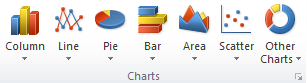
\includegraphics[max width=\linewidth]{../img/panel_charts.png}
\end{center}

\item Set the chart design (data serie to plot, order, etc.). You can use the ribbon's \texttt{Design} tab.

\begin{center}
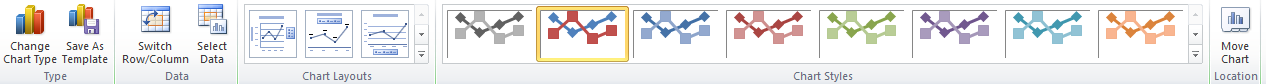
\includegraphics[max width=\linewidth]{../img/excel_2010_chart_design_ribbon.png}
\end{center}

\item Apply a layout (title, axis, legend, grids, data labels, etc.). You can use the ribbon's \texttt{Layout} tab.

\begin{center}
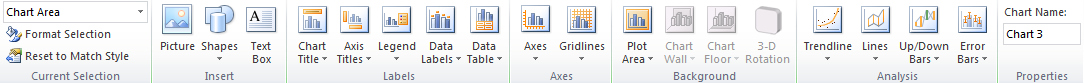
\includegraphics[max width=\linewidth]{../img/excel_2010_chart_layout_ribbon.png}
\end{center}

\item Apply a style format (text, line and background colours). You can use the ribbon's \texttt{Format} tab.

\begin{center}
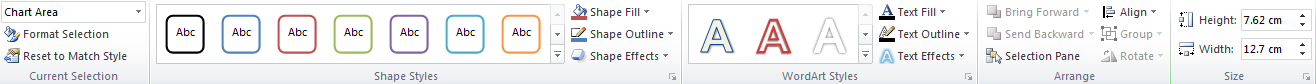
\includegraphics[max width=\linewidth]{../img/excel_2010_chart_format_ribbon.png}
\end{center}
\end{enumerate}

Charts are embedded in the same worksheet that data by default but it's possible to put it on a separate worksheet. For that right-clicking the chart background and select \texttt{Move chart}. In the dialog that appears select \texttt{New sheet} give a name to the worksheet a click OK.

Charts are linked to data from which they come. This means that any change in the data will be immediately reflected in any derived chart.

\section{Types of charts}\hypertarget{types-of-charts}{}\label{types-of-charts}

There are eleven major chart types (Column, Line, Pie, Bar, Area, Scatter, Stock, Surface, Doughnut, Bubble and Radar) and each has many subtypes.

Each chart type has a purpose and requires data to be arranged in a particular way. So choosing the right chart is probably the most important decision. The main chart types and their purpose are presented below.

\subsection{Column and bar charts}\hypertarget{column-and-bar-charts}{}\label{column-and-bar-charts}

A \href{https://en.wikipedia.org/wiki/Bar\_chart}{column or bar chart} is a set of bars (usually rectangles) graphed over an horizontal and vertical axis (also known as XY axis). Each bar is graphed over the corresponding category with a length proportional to the value of the category in the data serie. Usually more than one data serie are plotted and bars corresponding to different series are differentiated with colours. In a column chart, categories appear horizontally and values appear vertically, whereas in a bar chart, categories appear vertically.
Column charts, unlike bar charts, is suitable for emphasizing data variations over a period of time.

\textbf{Example}. The figure~\ref{img-example_chart_column} shows a column chart showing the evolution of fruit prices.
Looking at the chart you can quickly realize that strawberries are the most expensive (longest bars) and apples the cheapest (shortest bars) along the time. Also that the prices of strawberries and bananas are decreasing, the prices of oranges are increasing and the prices of apples are almost stables.

\begin{figure}[htbp]
\begin{center}
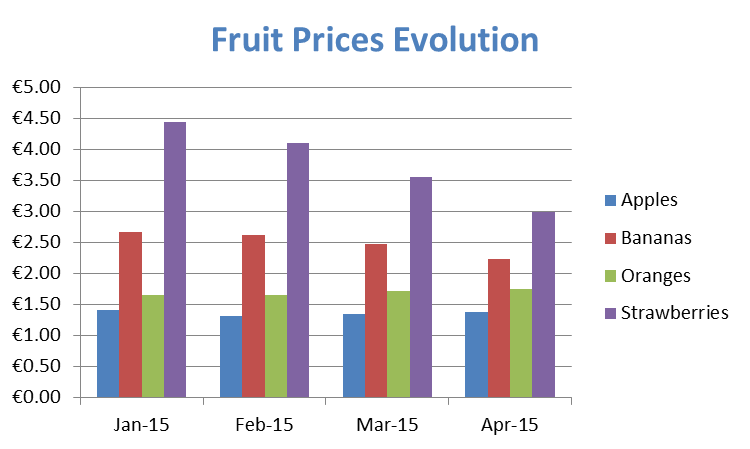
\includegraphics[scale=0.7]{../img/example_chart_column.png}
\end{center}
\caption{Example pie chart comparing fruit prices.}
\label{img-example_chart_column}
\end{figure}

Excel offers a lot of shapes for the bars (rectangles, cylinders, cones, pyramids) in 2-D an 3-D, and allows to stack bars. Also is possible to add error bars to the bars.

\textbf{Example}. This \href{http://aprendeconalf.es/office/excel/manual/img/example_chart_column_one_serie.gif}{animation} shows how to create a column chart for the apple prices evolution (one data serie).

And this \href{http://aprendeconalf.es/office/excel/manual/img/example_chart_column_several_series.gif}{animation} shows how to create a column chart for the fruit prices evolution (several data series).


\subsection{Line charts}\hypertarget{line-charts}{}\label{line-charts}

A \href{https://en.wikipedia.org/wiki/Line\_chart}{line chart} display a serie of data points called \emph{markers} connected by straight line segments. Each marker is graphed over the corresponding category at a height proportional to the value of the category in the data serie. It's similar to a column chart but using markers at the end of bars instead of bars, and joining them with straight line segments. Line charts are suitable for displaying and comparing trends over a period of time.

\textbf{Example}. The figure~\ref{img-example_chart_line} shows a line chart showing the evolution of fruit prices. Looking at the
chart you can quickly realize that strawberries are the most expensive (higher markers) and apples the cheapest (lowest markers) along the time. Also that the prices of strawberries and bananas are decreasing (lines with negative slope), the prices of oranges are increasing (line with positive slope) and the prices of apples first decrease an then increases.

\begin{figure}[htbp]
\begin{center}
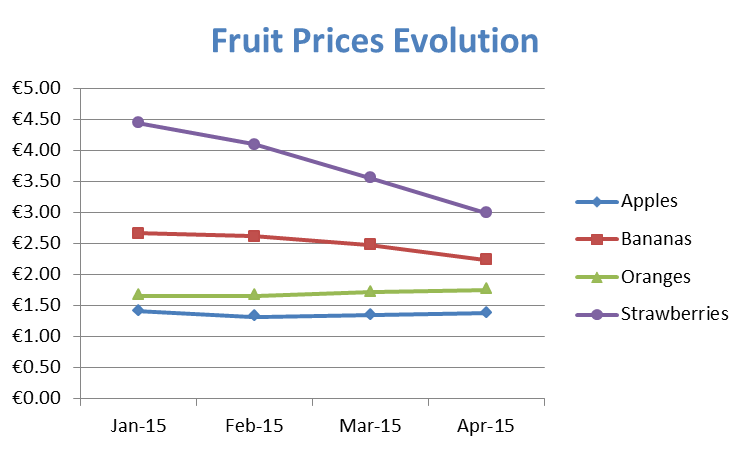
\includegraphics[scale=0.7]{../img/example_chart_line.png}
\end{center}
\caption{Example pie chart comparing fruit prices.}
\label{img-example_chart_line}
\end{figure}

Excel offers different subtypes of line charts, with or without data points in 2-D and 3-D, and also allows to stack lines.

\textbf{Example}. This \href{http://aprendeconalf.es/office/excel/manual/img/example_chart_line.gif}{animation} shows how to create a line chart for the fruit prices evolution. Looking at the chart you can quickly realize which prices are increasing and which prices are decreasing.

\subsection{Area charts}\hypertarget{area-charts}{}\label{area-charts}

An \href{https://en.wikipedia.org/wiki/Area\_chart}{area chart} is similar to a line chart but filling the area between the line and the horizontal axis. 
Area charts are suitable for displaying the relative importance of values over time. It'ss similar to a line chart, but because the area between lines is filled in, the area chart puts greater emphasis on the magnitude of values and less emphasis on the flow of change over time.

\textbf{Example}. The figure~\ref{img-example_chart_area} shows an area chart showing the evolution of accumulated fruit prices.
Looking at the chart you can quickly realize that strawberries are the most expensive (the largest area) and that
accumulated prices are decreasing. 

\begin{figure}[htbp]
\begin{center}
\includegraphics[scale=0.7]{../img/example_chart_area.png}
\end{center}
\caption{Example pie chart comparing fruit prices.}
\label{img-example_chart_area}
\end{figure}

Excel allows to plot areas in 2-D or 3-D and also to stack areas.

\textbf{Example}. This \href{http://aprendeconalf.es/office/excel/manual/img/example_chart_area.gif}{animation} shows how to create an area chart for the evolution of accumulated fruit prices.

\subsection{Pie charts}\hypertarget{pie-charts}{}\label{pie-charts}

A \href{https://en.wikipedia.org/wiki/Pie\_chart}{pie chart} is a circle divided into slices called \emph{sectors}. Each sector represents a category of the data serie an has an angle or area proportional to the quantity that correspond to the category.

Pie charts are suitable for displaying the parts of a whole. Unlike the other charts presented so far, which can graph multiple data series, pie charts can graph just one data series.

\textbf{Example}. The figure~\ref{img-example_chart_pie} shows a pie chart comparing fruit prices. Looking at the chart you can
quickly realize that strawberries are the most expensive (biggest sector) and apples are the cheapest (smallest sector).

\begin{figure}[htbp]
\begin{center}
\includegraphics[scale=0.7]{../img/example_chart_pie.png}
\end{center}
\caption{Example of pie chart comparing fruit prices.}
\label{img-example_chart_pie}
\end{figure}

Again Excel has several subtypes that allows you to emphasize a part of the whole in 2-D or 3-D.

\textbf{Example}. This \href{http://aprendeconalf.es/office/excel/manual/img/example_chart_pie.gif}{animation} shows how to create a pie chart comparing the fruit prices of January.

\subsection{Doughnut charts}\hypertarget{doughnut-charts}{}\label{doughnut-charts}

\href{https://en.wikipedia.org/wiki/Pie\_chart\#Doughnut\_chart}{Doughnut charts} are similar to pie charts except for its ability to display more than one data series.

\textbf{Example}. The ~\ref{img-example_chart_doughnut} shows a doughnut chart comparing fruit prices in January and April. The inner
doughnut correspond to prices of January and the outer to prices of April. Looking at the chart you can quickly realize that, although the price of apples were smaller in April than in January, it was relatively higher in April than in January, compared to the rest of fruit prices.

\begin{figure}[htbp]
\begin{center}
\includegraphics[scale=0.7]{../img/example_chart_doughnut.png}
\end{center}
\caption{Example of doughnut chart comparing fruit prices.}
\label{img-example_chart_doughnut}
\end{figure}

\textbf{Example}. This \href{http://aprendeconalf.es/office/excel/manual/img/example_chart_doughnut.gif}{animation} shows how to create a doughnut chart comparing the fruit prices in January and April.

\subsection{XY Scatter charts}\hypertarget{xy-scatter-charts}{}\label{xy-scatter-charts}

An \href{https://en.wikipedia.org/wiki/Scatter\_plot}{XY scatter chart} is a point cloud graphed using Cartesian coordinates. Each point correspond to a pair of values. The first value of the pair determines the position on the horizontal axis and the second value of the pair determines the position on the vertical axis. XY Scatter charts are suitable for displaying correlation among the data pairs of two numeric variables.

\textbf{Example}. The figure~\ref{img-example_chart_scatter} shows an XY Scatter chart relating banana and strawberry prices. Looking at
the chart you can quickly realize that there is a positive correlation (when banana price increase, strawberry price increase too).

\begin{figure}[htbp]
\begin{center}
\includegraphics[scale=0.7]{../img/example_chart_scatter.png}
\end{center}
\caption{Example of XY scatter chart relating banana and strawberry prices.}
\label{img-example_chart_scatter}
\end{figure}

\textbf{Example}. This \href{http://aprendeconalf.es/office/excel/manual/img/example_chart_scatter.gif}{animation} shows how to create an XY Scatter chart relating banana and strawberry prices.

\subsection{Histograms}\hypertarget{histograms}{}\label{histograms}

A \href{https://en.wikipedia.org/wiki/Histogram}{histogram} is a graphical representation of the distribution of numerical data. It's similar to a column chart but data values are grouped into interval classes and each bar represents a class. Histograms charts are suitable for displaying frequency of data values in one numeric variable.

To plot an histogram previously is required to load the \texttt{Analysis ToolPak} add-in.

\textbf{Example}. This \href{http://aprendeconalf.es/office/excel/manual/img/example_chart_histogram.gif}{animation} shows how to create an histogram of the grades in a course.

\section{Chart design}\hypertarget{chart-design}{}\label{chart-design}

\subsection{Changing the data source}\hypertarget{changing-the-data-source}{}\label{changing-the-data-source}

You can change the data range graphed in a chart anytime clicking the \texttt{Select Data} button of the \texttt{Data} panel on the ribbon's \texttt{Design} tab. This brings a dialog where you can select the new data range, switch rows and columns series, add new data series to graph and their labels, remove or edit existing data series or change the order in which are graphed in the chart.

Observe that is possible to plot in the same chart data in separated ranges.

\textbf{Example}. This \href{http://aprendeconalf.es/office/excel/manual/img/example_chart_add_data_serie.gif}{animation} shows how to add the orange prices data serie to a column chart for the apple prices evolution.

\subsection{Switching rows and columns}\hypertarget{switching-rows-and-columns}{}\label{switching-rows-and-columns}

When Excel creates a new chart with x and y axis, it automatically graphs the data by rows in the selected range so that the column headings appear along the horizontal axis and the row headings appear in the legend. If you want to switch from row series to column series, that is, that row headings appear on the horizontal axis and the column headings appear in the legend, click the \texttt{Switch Row/Column} button of the \texttt{Data} panel on the ribbon's \texttt{Design} tab.

\textbf{Example}. This \href{http://aprendeconalf.es/office/excel/manual/img/example_chart_switch_row_column.gif}{animation} shows how to switch from row series to column series in a column chart for the fruit prices evolution.

\section{Chart layout}\hypertarget{chart-layout}{}\label{chart-layout}

After creating a chart you can add new layout elements like chart titles, axis titles, legends, data labels, grids, trend lines, error bars, etc. or modify the existing ones.

\begin{figure}[htbp]
\begin{center}
\includegraphics[scale=0.7]{../img/chart_parts.png}
\end{center}
\caption{Parts of a chart.}
\label{img-chart_parts}
\end{figure}

To format any element of a chart right-click the element (bar, line, title, axis, legend, etc) and select the corresponding option at the bottom of the contextual menu. This will open a dialog where you can perform the desired changes for the selected element.

\subsection{Titles}\hypertarget{titles}{}\label{titles}

You can add a title to the chart selecting the chart and clicking the \texttt{Chart Title} button of the \texttt{Labels} panel on the ribbon's \texttt{Layout} tab. That will show a drop down menu that let you choose between a centered overlay title (inside the chart area) or an above chart (outside the chart area).

\textbf{Example}. This \href{http://aprendeconalf.es/office/excel/manual/img/example_chart_title.gif}{animation} shows how to add a title to a column chart for the fruits prices evolution and how to change the font colour.

\subsection{Axes}\hypertarget{axes}{}\label{axes}

You can add a title to the horizontal or vertical axes selecting the chart and clicking the \texttt{Axis Title} button of the \texttt{Labels} panel on the ribbon's \texttt{Layout} tab.

\textbf{Example}. This \href{http://aprendeconalf.es/office/excel/manual/img/example_chart_axis_title.gif}{animation} shows how to add a title to the horizontal and vertical axes of a column chart for the fruits prices evolution. The vertical axis title is rotated 90 degrees.

One of the most important parts of a chart are axis scales. Excel allows you to configure the axis scale setting the minimum and maximum showed in the axis, the major and minor units, the format of thick marks (small lines intersecting axis that indicate categories, scale units or chart data series) and their labels, or even the scale type (linear by default or logarithmic). To configure an axis right-click any label of the axis (not the axis title) and select the \texttt{Format Axis} option from the contextual menu. This will open a dialog with a lot of axis options. Change whatever you want and click Close.

\textbf{Example}. This \href{http://aprendeconalf.es/office/excel/manual/img/example_chart_axis_scale.gif}{animation} shows
how to change the scales of the horizontal and vertical axes of a column chart for the apple prices evolution.
Observe that in the original chart the minimum value of the vertical axis scale is 1.26, what magnify the differences between month prices. To avoid that the minimum value of vertical scale is set to €0, and the major unit is set to €0.1. Also the format of tick marks labels is changed to currency with two decimal places. On the other hand, the tick marks labels of the horizontal axis are rotated 30 degrees counterclockwise.


\subsection{Grid}\hypertarget{grid}{}\label{grid}

A grid is composed of horizontal or vertical lines (usually equally spaced) over the axes. Grids are helpful to mark out more precisely the position of markers, bars, lines or other chart elements in the axis scales.

Excel allows to plot both horizontal and vertical grid lines for major and minor tick marks. To plot vertical grid lines right-click any label of the horizontal axis and select the \texttt{Add Major Gridlines} option for drawing lines over the major tick marks, or \texttt{Add Minor Gridlines} for drawing lines over the minor tick marks. To plot horizontal grid lines do the same but right-clicking any label of the vertical axis. Once the grid line is plotted you can change its format right-clicking any label of the axis and selecting the \texttt{Format Major Gridlines} or \texttt{Format Minor Gridlines} option.

\textbf{Example}. This \href{http://aprendeconalf.es/office/excel/manual/img/example_chart_grid.gif}{animation} shows how add vertical major grid lines and horizontal minor grid lines. Also show how to change the line style of minor grid lines.

\subsection{Legends}\hypertarget{legends}{}\label{legends}

A legend is key that identifies patterns, colors, or symbols associated with the markers of a chart data series. The legend shows the data series name corresponding to each data marker.

Excel usually plots a legend to the right of the chart but it's possible to change the legend to other position or to remove it. To plot the lenged of a chart click the \texttt{Legend} button of the \texttt{Labels} panel on the ribbon's \texttt{Layout} tab. This shows a drop down menu with different positions for the legend. After plotting the legend, if you want to format it right-click it and select \texttt{Format Legend}. This will open a dialog where you can choose the legend position, the frame and background colours and many other legend aspects. Finally if you want to remove a legend, just select it and press the \texttt{Supr} key.

\textbf{Example}. This \href{http://aprendeconalf.es/office/excel/manual/img/example_chart_legend.gif}{animation} shows how add a legend for the fruits to the right of a column chart with the fruit prices evolution. Also it shows how to plot a frame around the legend and how to move the legend to the top.

\subsection{Data series}\hypertarget{data-series}{}\label{data-series}

The aspect of any graphic element used to represent a data serie in a chart (bars, markers, lines, sectors, etc) can be easily changed. To format the graphic element corresponding to a data serie right-click it and select the \texttt{Format Data Series} option. This will open a dialog where you can change the shape, border and background colours, space between elements, and many other aspects. It's also possible to format only one element of the serie. For that you need to click it two times (not double-clicking), then right-click it and select the \texttt{Format Data Point} option.

\textbf{Example}. This \href{http://aprendeconalf.es/office/excel/manual/img/example_chart_data_series.gif}{animation} shows how to change the background colour of orange bars in a column chart for the fruits prices evolution. It also shows how to add a glow effect over the highest bar.

\subsection{Data labels}\hypertarget{data-labels}{}\label{data-labels}

Sometime is useful to plot the values for a data serie next to their bars, markers, lines, sectors or other chart elements. To plot the values of a data serie right-click the chart element (bar, marker, line, sector, etc) corresponding to the data serie and select the \texttt{Data Labels} option. This will plot the value corresponding to each bar, marker, sector, etc. close to it.

\textbf{Example}. This \href{http://aprendeconalf.es/office/excel/manual/img/example_chart_data_labels.gif}{animation} shows how add a legend for the fruits to the right of a column chart with the fruit prices evolution. Also it shows how to plot a frame around the legend and how to move the legend to the top.

\subsection{Chart styles}\hypertarget{chart-styles}{}\label{chart-styles}

Finally, the \texttt{Chart styles} panel on the ribbon's \texttt{Design} tab has many predefined chart styles that combine different colours for graphics elements and backgrounds. Apply one of those styles is as easy as select the chart an click the desired style.

Also, the \texttt{Shape styles} panel on the ribbon's \texttt{Format} tab have predefined styles for the background area and frame of the chart.

\textbf{Example}. This \href{http://aprendeconalf.es/office/excel/manual/img/example_chart_styles.gif}{animation} shows how to apply some chart and shape styles to a column chart with the fruit prices evolution.

 
% Autor: Alfredo Sánchez Alberca (email:asalber@ceu.es)

\chapter{Managing databases}

A \href{https://en.wikipedia.org/wiki/Database}{database} is an organised collection of data. Usually databases are composed of records that contains information about the same object (person, company, product, etc), and records are composed of fields that contains every piece of information (name, address, phone number, price, etc.).

\textbf{Example} The next table show a students database with fields \emph{First name, Last name, Address, City, Birth date, Average grade} and \emph{Passed credits}.

\noindent\resizebox{\linewidth}{!}{ 
\begin{tabular}{|l|l|l|l|c|r|r|} 
\hline
First name & Last name & Address & City & Birth date & Average grade & Passed credits\\
\hline
María & Sánchez García & c. Estrella, 9 & Madrid & 23/10/1994 & 5,8 & 78\\
Carlos & Pérez López & c. Bravo Murillo, 34 3º-D & Madrid & 16/08/1993 & 7,9 & 123\\
Luis & González Roca & c. Antonio López, 67 1º-A & Madrid & 07/07/1995 & 8,2 & 45\\
Camen & Aguirre Jordán & c. Espada, 12 4º-C & Sevilla & 06/03/1994 & 4,2 & 28\\
Luisa & Martín Garrido & c. Cervantes, 14 & Albacete & 22/01/1994 & 6,7 & 54\\
Alberto & Pintado Marín & c. Arroyo, 27 2º-C & Sevilla & 10/03/1995 & 4,1 & 12\\
Marina & Gómez Gómez & c. Velázquez 28 4º-A & Madrid & 12/04/1994 & 7,7 & 62\\
Javier & Yagüe Pinzón & c. Rosales, 76 8º-B & Madrid & 18/12/1993 & 6,1 & 82\\
Lucas & Guerrero Monzón & c. Isaac Peral, 30 Bajo & Albacete & 12/01/1995 & 5,4 & 32\\
\hline
\end{tabular}
}

\section{Database creation in Excel}\hypertarget{database-creation-in-excel}{}\label{database-creation-in-excel}

Excel allows to define databases as tables where fields are defined in columns and records in rows. The first row of the table contains labels for each field. This tables are also called \emph{data lists}.

To create a data list first enter the name of the fields in the first row of the table, each in one column. This first row with the field names is the \emph{headers row}. Field names must be unique and there musn't be blank cells in the headers row. After creating the fields enter first record data in the appropriate columns of the row immediately below the one containing the field names. To Excel recognise this table as a data list, click the \texttt{Format as Table} button on the ribbon’s \texttt{Home} tab and then click a thumbnail of one of the table styles in the drop-down gallery.

After that you can enter the remaining records, one by row. After entering the data of a field press the \texttt{Tab} key to go to the next field of the same record, or to the first field of the next record if you are in the last field of a record.

\textbf{Example}. This \href{http://aprendeconalf.es/office/excel/manual/img/example_database_creation.gif}{animation} shows how create a data list of students with the fields \emph{First name, Last name, Address, City, Birth date, Average grade} and \emph{Passed credits}.

After creating a data list Excel will give a name to it, but is advisable to give it a descriptive name (see the \href{/office/excel/manual/formulas.html\#Namingcellsandranges}{Naming cells and ranges} section).

\section{Data validation}\hypertarget{data-validation}{}\label{data-validation}

When entering data to a data list is important to validate data to maintain database integrity. Data validation allows to specify which type and range of data are accepted by a cell or field (column). To apply a validation rule to a field, select the field column of the data list and click \texttt{Data validation} button of the \texttt{Data tools} panel on the ribbon's \texttt{Data} tab. In the dialog that appears, select the validation criteria from the drop-down list of the \texttt{Setting}:

\begin{itemize}
\item \emph{Whole number} allows only integers numbers between a specified minimum and a maximum or greater o less than a specified number.
\item \emph{Decimal} allows decimal numbers between a specified minimum and maximum or greater or less than a specified number.
\item \emph{List} allows a list of defined entries.
\item \emph{Date} allows dates between two specified dates or before or after a specified date.
\item \emph{Time} allows times between two specified times or before of after a specified time.
\item \emph{Text length} allows text with a restricted length.
\end{itemize}

After selecting the validating criteria, enter the correspondent parameters (minimum or maximum numbers, dates, times or range with the entries of the list). You can also define an input message in the \texttt{Input Message} tab and an error message in the \texttt{Error Alert} tab that will be shown if an invalid entry is entered in the field.

\textbf{Example}. This \href{http://aprendeconalf.es/office/excel/manual/img/example_data_validation.gif}{animation} shows how create a validation rule for the \emph{Average grade} field in a data list of students.

\section{Importing databases}\hypertarget{importing-databases}{}\label{importing-databases}

Excel offers the possibility to import data from diverse sources like csv text files, XML files, relational databases like Access or web data sources.

\subsection{Importing data from csv text files}\hypertarget{importing-data-from-csv-text-files}{}\label{importing-data-from-csv-text-files}

To see how to import data from csv text file see the section~\ref{import-from-csv-format}.

\subsection{Importing from web data sources}\hypertarget{importing-from-web-data-sources}{}\label{importing-from-web-data-sources}

There are many web pages that offers open data in a suitable format for import from Excel. To import data from a web data source click the \texttt{From Web} buttom of the \texttt{Get External Data} panel on the ribbon's \texttt{Data} tab. This opens a web browser where you must enter the URL of the page with de data source. When the browser shows the data table some yellow arrows appears that allow you to select the rows and columns of the table to import.

\textbf{Example} This \href{http://aprendeconalf.es/office/excel/manual/img/example_import_web.gif}{animation} shows how to import the IBEX 35 serie from \href{https://es.finance.yahoo.com/}{Yahoo finances}.

\subsection{Importing data from Qandl}\hypertarget{importing-data-from-qandl}{}\label{importing-data-from-qandl}

\href{https://www.quandl.com/}{Quandl} is a finance and economic data repository with hundred of open data series. It's possible to import data from Qandl to Excel easily, but you need the Quandl add in for Excel. To install the Quandl add in for Excel follow these \href{https://www.quandl.com/help/excel}{instructions}.

After installing the add in a new tab labelled \texttt{Quandl} appears in the ribbon. To import a data serie from Qandl, first search the data serie clicking the \texttt{Search} button on the ribbon's \texttt{Quandl} tab, enter some key words for the search and click the \texttt{Show Results} button, select the data serie desired from the search results, click the \texttt{Insert Selected Codes} buttom and click the \texttt{Close} button. This will insert the Quandl code of the data serie (if you know the Quandl code of the data serie you can avoid the search and enter it directly in a cell). Finally, select the cell with the Quandl code and click the \texttt{Download} button on the ribbon's \texttt{Quandl} tab. This will download the data serie and put it in a range below the cell that contais the Quandl code.

\textbf{Example} This \href{http://aprendeconalf.es/office/excel/manual/img/example_import_quandl.gif}{animation} shows how to import the IBEX 35 serie from \href{https://www.quandl.com/}{Quandl}.

\section{Data sorting}\hypertarget{data-sorting}{}\label{data-sorting}

To sort the data list records on a single field, you simply click that field’s \texttt{AutoFilter} button (the button with the triangle that appears to the right of the header) and then click the appropriate sort option on its drop-down list:
- Sort A to Z or Sort Z to A in a text field.
- Sort Smallest to Largest or Sort Largest to Smallest in a number field.
- Sort Oldest to Newest or Sort Newest to Oldest in a date field.

Other option to sort a data list on a field is to select a cell of the field column an click the \texttt{Sort A to Z}
button \includegraphics[scale=0.7]{../img/button_az.png}  of the \texttt{Sort \& Filter} panel on the ribbon’s
\texttt{Data} tab, to sort ascending, or the \texttt{Sort Z to A} button
\includegraphics[scale=0.7]{../img/button_za.png} to sort descending.

Excel then will reorder all the records in the data list according to the ascending or descending order selected.

\textbf{Example}. This \href{http://aprendeconalf.es/office/excel/manual/img/example_database_sorting.gif}{animation} shows how to sort a students database. First ascending on the \emph{Birth date} field, next descending on the \emph{Average degree} field, and finally ascending on the \emph{Last name} field.

If you need to sort a data list on more than one field, select a cell of the data list and click the \texttt{Sort} button of the \texttt{Sort \& Filter} panel on the ribbon's \texttt{Data} tab. Then, in the dialog that appears, select the first sorting field column and the sorting order (ascending or descending), next the second sorting field column an the sorting order, and so on.

\textbf{Example}. This \href{http://aprendeconalf.es/office/excel/manual/img/example_database_sorting_on_multiple_fields.gif}{animation} shows how to sort a students database on the fields \emph{City} ascending and \emph{Average grade} descending.

You can also sort a range of cells in general indicating the name of the columns instead of the field names.

\section{Summarizing data}\hypertarget{summarizing-data}{}\label{summarizing-data}

With large tables or data lists is difficult to extract relevant information. For that purpose, Excel provides several methods for summarizing data.

\subsection{Totaling and subtotaling fields}\hypertarget{totaling-and-subtotaling-fields}{}\label{totaling-and-subtotaling-fields}

A common operation is to apply a function to a whole field in a data list, as for instance the SUM function for summarizing or the AVERAGE function for averaging all the values in a field column. This could be done activating the \texttt{Total row} check box of the \texttt{Table Style Options} panel on the ribbon's \texttt{Table Options} tab. This will add a total row at the bottom of the table. Clicking any cell of this row you can choose which function to apply to the whole field.

\textbf{Example} This \href{http://aprendeconalf.es/office/excel/manual/img/example_field_summarizing.gif}{animation} shows how to sum the passed credits of students in a students database. It also shows how to average the average grade.

Excel also allows subtotaling a field by categories of other field. This procedure only works with data lists formatted
like tables, so if a data list have been formatted like a table first it has to be converted to a range selecting any
cell of the table and clicking the \texttt{Convert to Range} button of the \texttt{Tool} panel on the ribbon's
\texttt{Table Tools - Design} tab. After that, you have to sort the data list by the field with the categories to
summarize (see the section~\ref{data-sorting}). Finally, to subtotaling a data list click the \texttt{Subtotal} button
of the \texttt{Outline} panel on the ribbons' \texttt{Data} tab. This will display a dialog where you have to select the field with the categories in the \texttt{At each change in} drop-down menu, the function to apply (sum, count, average, etc.) in the \texttt{Use function} drop-down menu, check the fields to with apply the subtotaling function in the \texttt{Add subtotal to} list, and click OK.

\textbf{Example} This \href{http://aprendeconalf.es/office/excel/manual/img/example_field_subtotaling.gif}{animation} shows how to subtotaling the passed credits of students in a students database by the city where they live.

\subsection{Pivot tables}\hypertarget{pivot-tables}{}\label{pivot-tables}

A pivot table is a powerful tool for exploring data. It help you organise and summarize the raw data in your data list, revealing patterns or relationships that might not be obvious at first glance.

To create a pivot table click on any cell of a data list and then click the \texttt{PivotTable} button on the ribbon’s \texttt{Insert tab}. This display a dialog where you can select the range for the pivot table (by default Excel select the whole data list) and choose between placing the pivot table in a new workbook (default) or in the same workbook (in this case you have to indicate in which cell). After click OK, a pane appears on the right side of the pane:

\begin{itemize}
\item \textbf{Report Filter} for the fields that enable you to page through the data
summaries shown in the actual pivot table by filtering out sets of data —
they act as the filters for the report. So, for example, if you designate the
Year Field from a data list as a Report Filter, you can display data summaries in the pivot table for individual years or for all years represented
in the data list.
\item \textbf{Column Labels} for the fields that determine the arrangement of data shown in the columns of the pivot table.
\item \textbf{Row Labels} for the fields that determine the arrangement of data shown in the rows of the pivot table.
\item \textbf{Values} for the fields whose data are presented and summarized in the body cells of the pivot table. By default Excel will use the SUM function to summarize values. To use another function click the field and select the \texttt{Value Field Settings} option in the menu that appears. In the dialog that appears just select the function that you want to use for summarizing and click OK.
\end{itemize}

\textbf{Example} This \href{http://aprendeconalf.es/office/excel/manual/img/example_pivot_table_1.gif}{animation} shows how to create a pivot table for a students database. The pivot table shows and summarizes the passed credits by degrees on rows and by cities on columns.

This \href{http://aprendeconalf.es/office/excel/manual/img/example_pivot_table_2.gif}{animation} shows how to arrange the previous pivot table to show the passed credits summarized first by city and then by degree and vice versa, both on rows.

This \href{http://aprendeconalf.es/office/excel/manual/img/example_pivot_table_3.gif}{animation} shows how to arrange the previous pivot table to show, in addition to the passed credits, the average grade of students. The passed credits are summarized using the SUM function while the average grade is summarized using the AVERAGE function.

This \href{http://aprendeconalf.es/office/excel/manual/img/example_pivot_table_4.gif}{animation} shows how to filter the previous pivot table to show only the values of course year 2014 and not to show the physics degree.

To change the format of a pivot table you can use the \texttt{Layout} panel on ribbon's \texttt{PivotTable Tools - Design} tab. This panel has four buttons:

\begin{itemize}
\item \textbf{Subtotals} Allows to show subtotals at top of groups, at bottom of groups or not to show subtotals.
\item \textbf{Grand Totals} Allows to show grand totals for rows, for columns, for both rows and columns, or not to show grand totals.
\item \textbf{Report Layout} Allows to show the groups in compact form (all the grouping fields in the same column), in outline form (every grouping field in a different column) or in tabular form (like the outline form but adding extra rows for the subtotals).
\item \textbf{Blank rows} Allow to insert or not a blank row after each group.
\end{itemize}

It's also possible to apply a predefined style to a pivot table just selecting the desired style from the \texttt{PivotTable Styles}  panel on ribbon's \texttt{PivotTable Tools - Design} tab.

\textbf{Example} This \href{http://aprendeconalf.es/office/excel/manual/img/example_pivot_table_formatting.gif}{animation} shows how to format and how to apply a style to the previous pivot table.

\subsection{Pivot chart}\hypertarget{pivot-chart}{}\label{pivot-chart}

Pivot tables can be accompanied by pivot charts, that is an interactive chart where you can present and summarize data grouped by some fields like a in a pivot table. To create a pivot chart from a pivot table, in the worksheet with the pivot table click the \texttt{PivotChart} button of the \texttt{Tools} panel on the ribbon's \texttt{PivotTable Tools - Options} tab. This will show a dialog with the charts types. Select the desired chart type and click OK. After that Excel inserts a chart in the same worksheet of the pivot table reflecting the same information of the pivot table. Fron now on, any change in the pivot table will be reflected in the pivot chart.

\textbf{Example} This \href{http://aprendeconalf.es/office/excel/manual/img/example_pivot_chart.gif}{animation} shows how to create a pivot chart from a pivot table for a students database.

Of course, you can change the pivot chart layout as any other chart (see section~\ref{chart-layout}).

\section{Data filtering}\hypertarget{data-filtering}{}\label{data-filtering}

With huge databases it's difficult to find the desired information. To overcome this problem Excel provide several methods to filter the database. Filtering is the procedure for specifying the data that you want displayed in an Excel data list.

\subsection{Apply a simple filter}\hypertarget{apply-a-simple-filter}{}\label{apply-a-simple-filter}

The easiest way to perform this basic type of filtering on a field is to click the \texttt{AutoFilter} button (the button with the triangle that appears to the right of the header). This display a drop-down menu that contains at the end a list box with a complete listing of all entries
made in that column, each with its own check box. In this list click the check box in front of the (Select All) option at the top of the field’s
list box to clear the check boxes, then click each of the check boxes corresponding to the entries for the records you do want displayed in the filtered data list, and finally click OK. Excel then hides rows in the data list for all records except for those that contain the entries you just selected.

\textbf{Example} This \href{http://aprendeconalf.es/office/excel/manual/img/example_database_filtering_simple.gif}{animation} shows how to filter the students of Sevilla and Albacete in a students database.

To perform more sophisticated filters you can use the other filter options of the \texttt{AutoFiller} button. These filter options depend on the type of entries in the field:

\begin{itemize}
\item If the column only contains dates, the menu contains a \texttt{Date Filters} option with a submenu that allows you to filter dates equals to, before o after a given date; dates between two given dates; dates of today, yesterday and tomorrow; dates of this week, last week and next week; dates of this month, last month and next month; dates of this quarter, last quarter and next quarter; dates of this year, last year and next year; and dates in a specific period (quarter or month).
\item If the column contains only numbers or a mixture of dates with numbers, the menu contains a \texttt{Number Filters} option with a submenu that allows you to filter numbers equal or not equal to a given number; numbers greater than, greater than or equal to, less than, less than or equal to a given number; numbers between two given numbers; top 10 numbers; number above the average and numbers below the average.
\item If the column only text or a mixture of text, date and numbers, the menu contains a \texttt{Text Filters} option with a submenu that allows you to filter text equal or not equal to a given text; text that begins or end with a given text; and text that contains or does not contains a given text.
\end{itemize}

If the filter selected requires some parameter (date, number or text), a dialog appears where you must enter that data and click OK.

\textbf{Example} This \href{http://aprendeconalf.es/office/excel/manual/img/example_database_filtering_complex.gif}{animation} shows how to filter the students born before 1/1/1995, with an average grade greater than or equal to 5, and whose name begins with M, in a students database.

\subsection{Apply a complex filter}\hypertarget{apply-a-complex-filter}{}\label{apply-a-complex-filter}

Simple filters are enough in most cases, but sometime you need to filter data according to more complex criteria. Fortunately Excel provides a method to perform filters based on calculated criteria with formulas.

To perform a filter with calculated criteria first you have to specify the criteria somewhere in the worksheet that
contains the data list. The criteria must have a cell header and a logical formula in the cell just below. In the
logical formula you can use functions and references to the cells, but it's important to note that all references must
be to cells in the first row of the data list. After that, to apply the filter you need to select a cell in the data
list and click the \texttt{Advanced} button \includegraphics[scale=0.7]{../img/button_advanced_filter.png} of the
\texttt{Sort \& Filter} panel on the ribbons's \texttt{Data} tab. This shows a dialog where you have to enter the range of the data list (usually Excel auto recognise it), the range of the filter criteria and click OK. Excel will apply the logical formula to every row of the data list and show only the records where the formula returns TRUE.

\textbf{Example} This \href{http://aprendeconalf.es/office/excel/manual/img/example_database_filtering_calculated_criteria.gif}{animation} shows how to filter the students with an average grade greater than or equal to 5, and a number of passed credits over the average, in a students database, using a calculated criteria. Observe how is used the data list name and the field name to reference the column of passed credits in the average calculation.

\subsection{Clear a filter}\hypertarget{clear-a-filter}{}\label{clear-a-filter}

To clear an active filter in a data list click the \texttt{AutoFilter} button of the column with the active filter and select the option \texttt{Clear Filter}. After that Excel will show all the records hidden by the removed filter, but the rest of filters will continue active. To clear all the filters in a data list, select a cell of the data list and then click the \texttt{Clear} button of the \texttt{Sort \& Filter} panel on the ribbons's \texttt{Data} tab. This will show all the records of the data list.

\section{Database functions}\hypertarget{database-functions}{}\label{database-functions}

Excel have some predefined functions that can be applied to data list. Some of them apply other function only to records in a data list that match a criteria you specify.

\subsection{Define a criteria}\hypertarget{define-a-criteria}{}\label{define-a-criteria}

The criteria must be defined in a range and must include at least one header with a field name that indicates the field whose values are to be evaluated and one cell just below with the value or expression to be used in the evaluation. The expression with the condition is a text string starting with a logical comparator (\texttt{=},\texttt{\textgreater{}},\texttt{\textless{}},\texttt{\textgreater{}=},\texttt{\textless{}=},\texttt{\textless{}\textgreater{}}) or a pattern text with wildcards like the question mark \texttt{?} (that matches any character) or the asterisk \texttt{*} (that matches any character string). You can specify multiple conditions in different columns. If you want to apply the function to all the records of the data list, just leave the cell with the criteria conditions blank.

\subsection{DSUM function}\hypertarget{dsum-function}{}\label{dsum-function}

The \texttt{DSUM} function sums the values in a numeric field (column) of records in a data list that match the criteria you specify. Its syntax is \texttt{DSUM(database,field,criteria)}, where \emph{database} is the range of the data list, \emph{field} is the name of the field that contains the values to add up (it must be a numeric column) enclosed in double quotes, and \emph{criteria} is the range that contains the criteria with the conditions you specify.

\textbf{Example} This \href{http://aprendeconalf.es/office/excel/manual/img/example_function_dsum.gif}{animation} shows how to sum the passed credits of students from Madrid born in 1994 or after with an average grade greater or equal to 6, in a students database.

\subsection{DCOUNT function}\hypertarget{dcount-function}{}\label{dcount-function}

The \texttt{DCOUNT} function counts the values in a numeric field (column) of records in a data list that match the criteria you specify. Its syntax is \texttt{DCOUNT(database,field,criteria)}, where \emph{database} is the range of the data list, \emph{field} is the name of the field that contains the values to add up (it must be a numeric column) enclosed in double quotes, and \emph{criteria} is the range that contains the criteria with the conditions you specify.

\textbf{Example} This \href{http://aprendeconalf.es/office/excel/manual/img/example_function_dcount.gif}{animation} shows how to count the students with an average grade greater than or equal to 6 whose name begins with L, in a students database.

\subsection{DMIN function}\hypertarget{dmin-function}{}\label{dmin-function}

The \texttt{DMIN} function returns the minimum in a numeric field (column) of records in a data list that match the criteria you specify. Its syntax is \texttt{DMIN(database,field,criteria)}, where \emph{database} is the range of the data list, \emph{field} is the name of the field that contains the values to add up (it must be a numeric column) enclosed in double quotes, and \emph{criteria} is the range that contains the criteria with the conditions you specify.

\subsection{DMAX function}\hypertarget{dmax-function}{}\label{dmax-function}

The \texttt{DMAX} function returns the maximum in a numeric field (column) of records in a data list that match the criteria you specify. Its syntax is \texttt{DMAX(database,field,criteria)}, where \emph{database} is the range of the data list, \emph{field} is the name of the field that contains the values to add up (it must be a numeric column) enclosed in double quotes, and \emph{criteria} is the range that contains the criteria with the conditions you specify.

\textbf{Example} This \href{http://aprendeconalf.es/office/excel/manual/img/example_function_dmin_dmax.gif}{animation} shows how to calculate the minimum and the maximum average grade of students from Madrid born before 1995, in a students database.

\subsection{DAVERAGE function}\hypertarget{daverage-function}{}\label{daverage-function}

The \texttt{DAVERAGE} function averages the values in a numeric field (column) of records in a data list that match the criteria you specify. Its syntax is \texttt{DAVERAGE(database,field,criteria)}, where \emph{database} is the range of the data list, \emph{field} is the name of the field that contains the values to add up (it must be a numeric column) enclosed in double quotes, and \emph{criteria} is the range that contains the criteria with the conditions you specify.

\textbf{Example} This \href{http://aprendeconalf.es/office/excel/manual/img/example_function_daverage.gif}{animation} shows how to average the average grades of students from Madrid born in 1994 or after with an average grade greater or equal to 6, in a students database.

\subsection{DSTDEVP function}\hypertarget{dstdevp-function}{}\label{dstdevp-function}

The \texttt{DSTDEVP} function calculates the standard deviation the values in a numeric field (column) of records in a data list that match the criteria you specify. Its syntax is \texttt{DSTDEVP(database,field,criteria)}, where \emph{database} is the range of the data list, \emph{field} is the name of the field that contains the values to add up (it must be a numeric column) enclosed in double quotes, and \emph{criteria} is the range that contains the criteria with the conditions you specify.

\textbf{Example} This \href{http://aprendeconalf.es/office/excel/manual/img/example_function_dstdevp.gif}{animation} shows how to calculate the standard deviation of average grades of students from Madrid born in Madrid before 1995, in a students database.

\subsection{DGET function}\hypertarget{dget-function}{}\label{dget-function}

The \texttt{DGET} returns the value of field (column) in the record of a data list that match the criteria you specify.
Its syntax is \texttt{DGET(database,field,criteria)}, where \emph{database} is the range of the data list, \emph{field}
is the name of the field that contains the values to return enclosed in double quotes, and \emph{criteria} is the range that contains the criteria with the conditions you specify.

If no record satisfy the criteria, the function returns a #VALUE! error, and if more than one records satisfy the
criteria the functions return a #NUM! error.  

\textbf{Example} This \href{http://aprendeconalf.es/office/excel/manual/img/example_function_dget.gif}{animation} shows how to find the student with the highest grade in a student database.
 
Other functions allow to search values in a list or table.

\subsection{VLOOKUP and HLOOKUP functions}\hypertarget{vlookup-and-hlookup-functions}{}\label{vlookup-and-hlookup-functions}

The \texttt{VLOOKUP} function finds things in a table or list by row. Its syntax is \texttt{VLOOKUP (value, table, col-index, [approx-match])}, where \emph{value} is the value you want to look up, \emph{table} is the range of the table or list in which to perform the search, \emph{col-index} is the the column number (starting with 1 for the left-most column of \emph{table} range) that contains the return value, and \emph{approx-match} is an optional logical argument that specifies whether to find an approximate match (TRUE by default) or an exact match (FALSE). The function looks the \emph{value} argument up in the first column of the \emph{table} argument. If the \emph{approx-match} argument is TRUE, the \emph{table} should be ordered by the firs column (the column where to look the \emph{value} up) and the function will return the value of the \emph{col-index} column in the same row that the closest value to \emph{value} in the first column of the \emph{table} range. If \emph{approx-match} is false, the function will search for the exact value in the firs column and it will return the value of the \emph{col-index} column in the same row that the first matched value in the first column. If no value in the first column matches the \emph{value} argument, the function will return a \#N/A error.

\textbf{Example} This \href{http://aprendeconalf.es/office/excel/manual/img/example_function_vlookup.gif}{animation} shows how to look the phone up of a student in a students database.

The \texttt{HLOOKUP} function works like the VLOOKUP function but it performs a search by columns. Its syntax is \texttt{HLOOKUP (value, table, row-index, [approx-match])}, where \emph{value} is the value you want to look up, \emph{table} is the range of the table or list in which to perform the search, \emph{row-index} is the the row number (starting with 1 for the top-most row of \emph{table} range) that contains the return value, and \emph{approx-match} is an optional logical argument that specifies whether to find an approximate match (TRUE by default) or an exact match (FALSE).

 
 
% % BIBLIOGRAPHY
% \printbibliography
% 
% % APENDIX
% \appendix
 
\end{document}


